\documentclass[
hidelinks,
12pt, % The default document font size, options: 10pt, 11pt, 12pt
oneside, % Two side (alternating margins) for binding by default, uncomment to switch to one side
english, % ngerman for German
doublespacing, % Single line spacing, alternatives: onehalfspacing or singlespacing
%draft, % Uncomment to enable draft mode (no pictures, no links, overfull hboxes indicated)
%nolistspacing, % If the document is onehalfspacing or doublespacing, uncomment this to set spacing in lists to single
%liststotoc, % Uncomment to add the list of figures/tables/etc to the table of contents
%toctotoc, % Uncomment to add the main table of contents to the table of contents
%parskip, % Uncomment to add space between paragraphs
%nohyperref, % Uncomment to not load the hyperref package
headsepline, % Uncomment to get a line under the header
%chapterinoneline, % Uncomment to place the chapter title next to the number on one line
%consistentlayout, % Uncomment to change the layout of the declaration, abstract and acknowledgements pages to match the default layout
]{MastersDoctoralThesis} % The class file specifying the document structure

\usepackage[utf8]{inputenc} % Required for inputting international characters
\usepackage[T1]{fontenc} % Output font encoding for international characters
\usepackage{subcaption}
\usepackage{mathpazo} % Use the Palatino font by default
\usepackage{booktabs}
\usepackage{colortbl}
\usepackage[final]{pdfpages}
\usepackage{xcolor}
\usepackage{balance}
\usepackage{epigraph}
\usepackage{alltt} % for code snippet
\usepackage{listings}
\usepackage{hyperref}
\usepackage{amsmath}
\usepackage{macros}
\usepackage{mathtools}
\usepackage{optidef}
\usepackage{float}
\usepackage{newtxmath}
\usepackage{polski}
\usepackage{tikz-cd}
\usepackage{flowchart}
\usetikzlibrary{
  shapes,
  arrows.meta, % supersedes arrows
  calc,automata,positioning,fit,quotes}
  \tikzset{
  line/.style={draw, -Latex}
}
\tikzstyle{arrow} = [thick,->,>=stealth]
\usepackage[backend=bibtex,style=authoryear,natbib=true]{biblatex} % Use the bibtex backend with the authoryear citation style (which resembles APA)
%\usepackage[backend=bibtex,style=authoryear,natbib=true,backref=true]{biblatex} % use this line instead of the previous one if you want to use back references

\addbibresource{biblio.bib} % The filename of the bibliography


\usepackage[autostyle=true]{csquotes} % Required to generate language-dependent quotes in the bibliography

%----------------------------------------------------------------------------------------
%	MARGIN SETTINGS
%----------------------------------------------------------------------------------------

\geometry{
	paper=a4paper, % Change to letterpaper for US letter
	inner=4.0cm, % Inner margin
	outer=3.0cm, % Outer margin
	bindingoffset=.5cm, % Binding offset
	top=2.5cm, % Top margin
	bottom=2.5cm, % Bottom margin
    head=23.99748pt,
	%showframe, % Uncomment to show how the type block is set on the page
}

%----------------------------------------------------------------------------------------
%	THESIS INFORMATION
%----------------------------------------------------------------------------------------

\thesistitle{Manifold Structure of High-Dimensional Data in\\ Artificial and Biological  Neural Networks} % Your thesis title, this is used in the title and abstract, print it elsewhere with \ttitle
\supervisor{Dr/Pr. FirstName \textsc{LastName}} % Your supervisor's name, this is used in the title page, print it elsewhere with \supname
\examiner{Dr/Pr. FirstName \textsc{LastName}} % Your examiner's name, this is not currently used anywhere in the template, print it elsewhere with \examname
\degree{B.Sc (Hons)} % Your degree name, this is used in the title page and abstract, print it elsewhere with \degreename
\author{\textsc{Zhang} Liu} % Your name, this is used in the title page and abstract, print it elsewhere with \authorname
\addresses{} % Your address, this is not currently used anywhere in the template, print it elsewhere with \addressname

\subject{Mathematical, Computational and Statistical Sciences} % Your subject area, this is not currently used anywhere in the template, print it elsewhere with \subjectname
\keywords{Manifold Learning, recurrent neural networks, computational vision, harmonic analysis} % Keywords for your thesis, this is not currently used anywhere in the template, print it elsewhere with \keywordnames
\university{\href{https://www.yale-nus.edu.sg/}{Yale-NUS College}} % Your university's name and URL, this is used in the title page and abstract, print it elsewhere with \univname
\department{{}} % Your department's name and URL, this is used in the title page and abstract, print it elsewhere with \deptname
\group{{}} % Your research group's name and URL, this is used in the title page, print it elsewhere with \groupname
\faculty{{}} % Your faculty's name and URL, this is used in the title page and abstract, print it elsewhere with \facname

\AtBeginDocument{
%\hypersetup{colorlinks=false}
\hypersetup{pdftitle=\ttitle} % Set the PDF's title to your title
\hypersetup{pdfauthor=\authorname} % Set the PDF's author to your name
\hypersetup{pdfkeywords=\keywordnames} % Set the PDF's keywords to your keywords
\hypersetup{hypertexnames=true}
}


%%% TODO NOTES 
\usepackage{todonotes}
\def\frs#1{\todo[color=green!30]{\textbf{FS}:#1}}
\def\frsi#1{\todo[color=green!30,inline]{\textbf{FS}:#1}}

\begin{document}

\frontmatter % Use roman page numbering style (i, ii, iii, iv...) for the pre-content pages

\pagestyle{plain} 

\begin{titlepage}
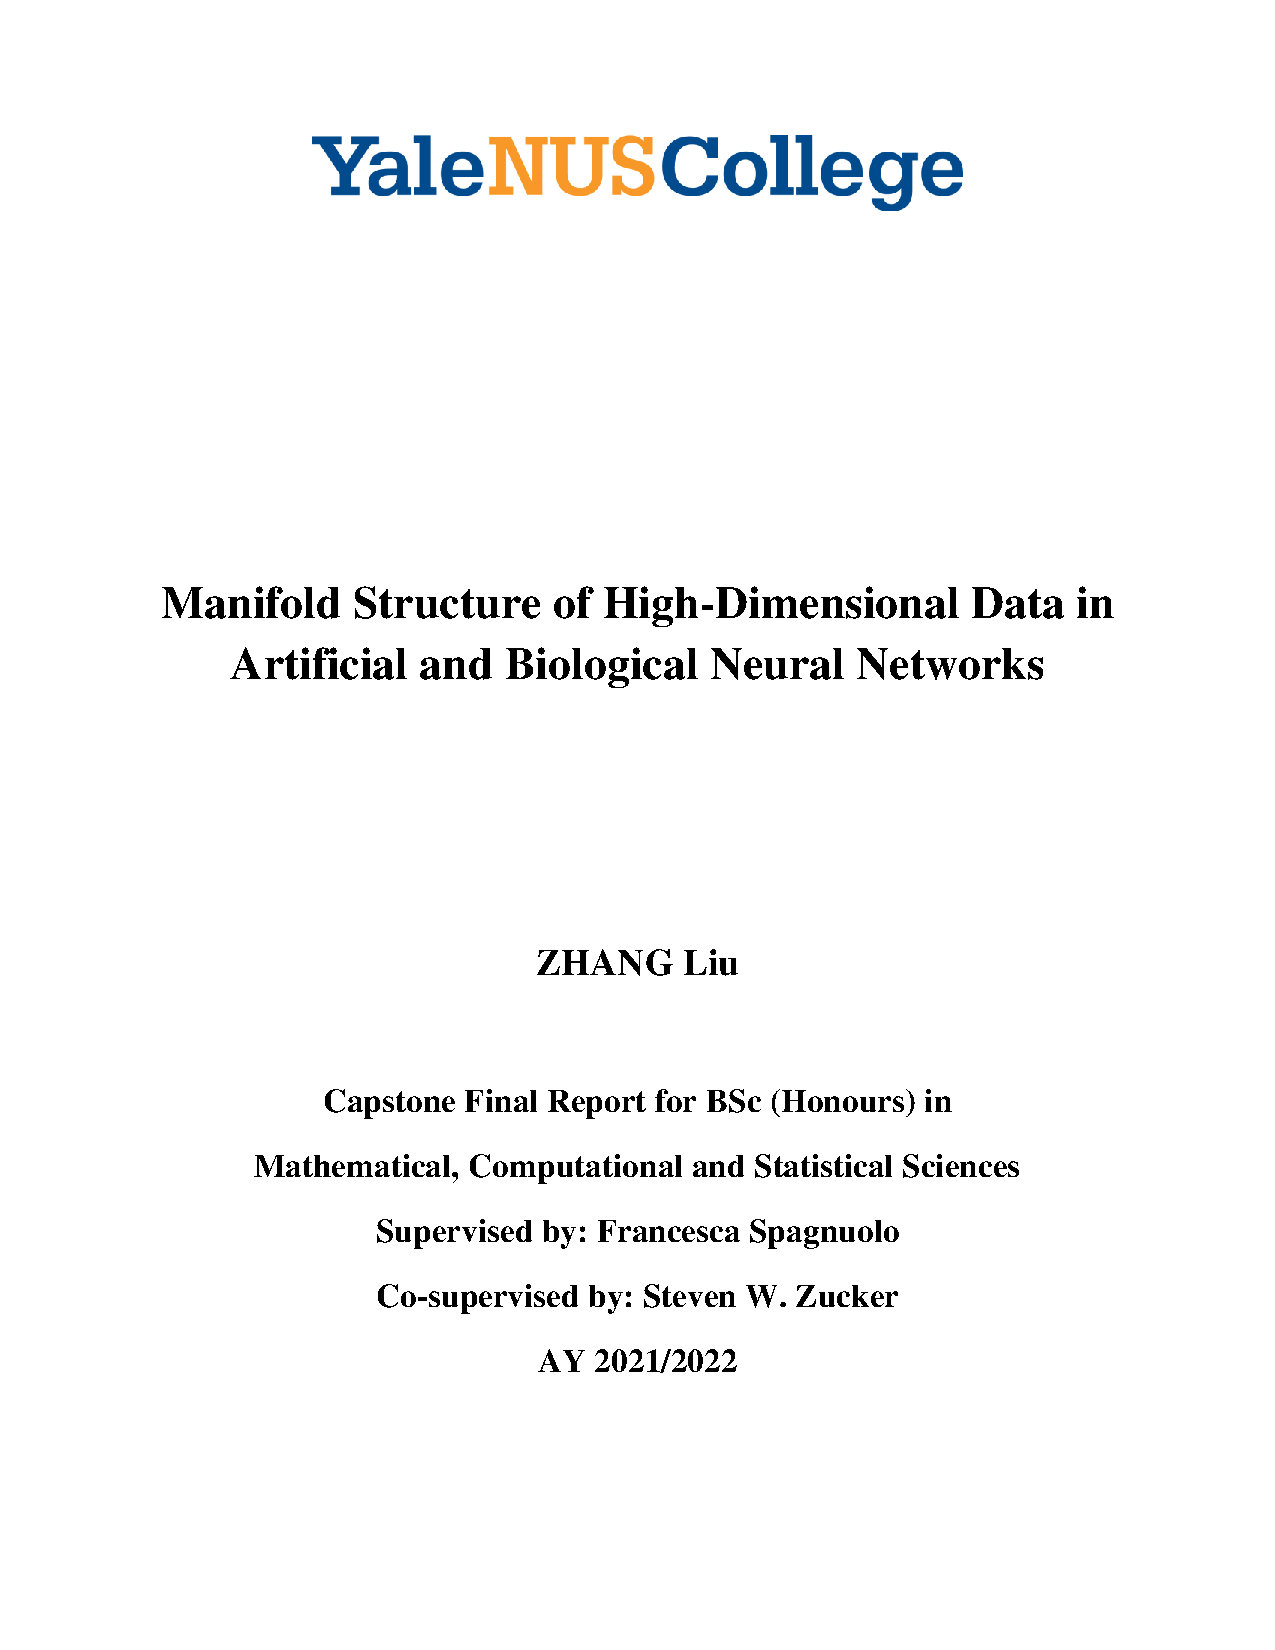
\includepdf[pages=-,pagecommand={},width=\textwidth]{capstone_titlepage.pdf}

\end{titlepage}

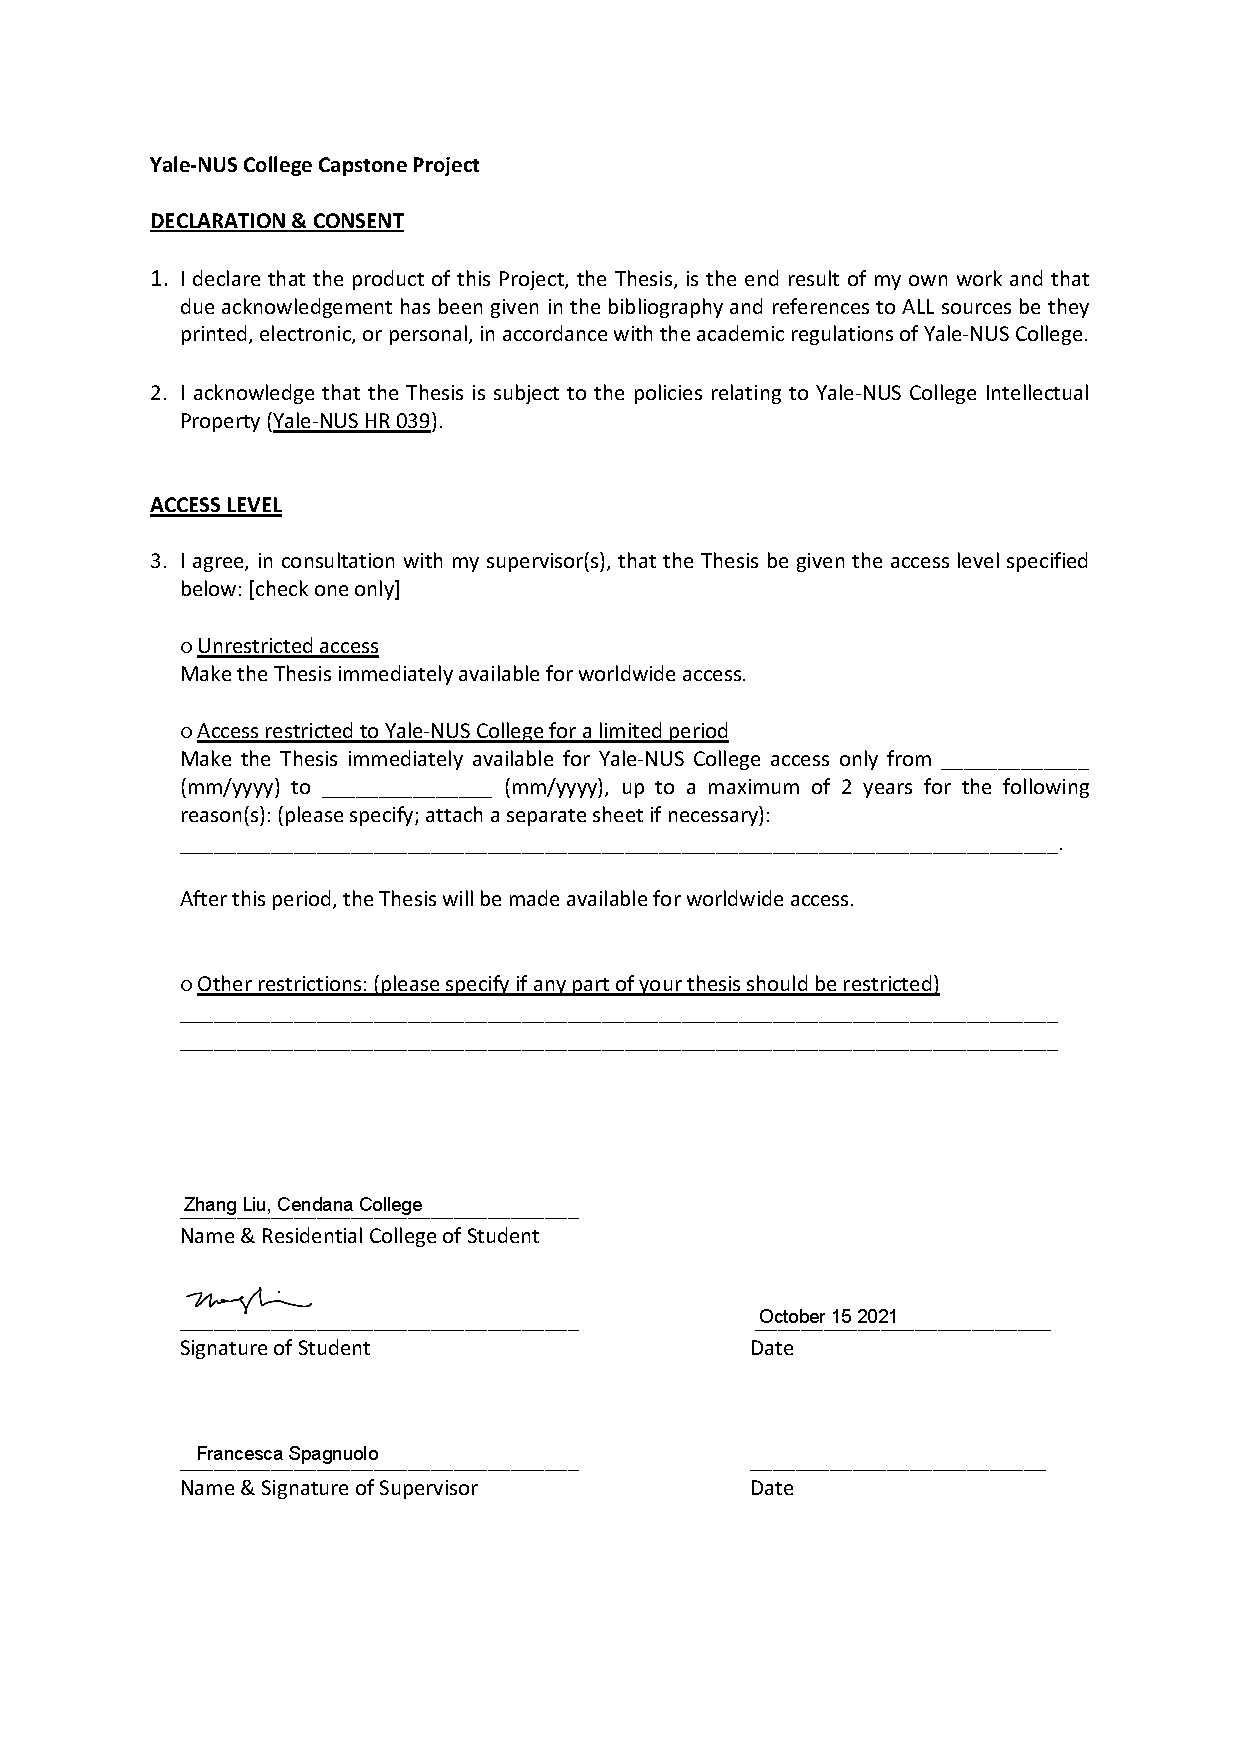
\includepdf[pages=-,pagecommand={},width=\textwidth]{declaration.pdf}

\begin{acknowledgements}
\addchaptertocentry{\acknowledgementname} % Add the acknowledgements to the table of contents
    I would like to thank my supervisor Prof.~Francesca Spagnuolo  and co-supervisor and mentor Prof.~Steven W. Zucker and Dr.~Luciano Dyballa for their generous guidance and advice. They have made possible the many serendipitous moments in this project.  There have been ups and downs in this project, but their support has helped me keep a keen spirit for learning and discovery. 
    
    I am also grateful for my family and friends who have been patiently bearing with my endless sharing of my work and ideas. 
\end{acknowledgements}

\begin{abstract}
\addchaptertocentry{\abstractname} % Add the abstract to the table of contents
\textbf{Key words: \keywordnames}

This work builds on a long line of research aiming to develop more accurate mathematical and computational models of the visual system. It has recently been shown that feed-forward neural networks turn out to be inaccurate models for the neurobiological networks in the visual cortex. We focused on a related question that has not been investigated: how is the structure of recurrent and transformer neural networks related to that of neurobiological networks (in the mouse visual cortex)?

We first build the biological and artificial neuron tensors using experimental neural spiking data and numerical simulations on recurrent and transformer neural networks. Using tensor component analysis, we discover which groups of neurons respond similarly to which stimuli input. Since these groups are likely not independent, we use the non-linear dimensionality reduction method, diffusion maps, to infer a manifold of neurons. This manifold structure implies a functional network (represented by the discrete data graph underlying the continuous manifold) and thus reflects both the neural circuit connections and the neuron’s role in those circuits. Comparing the manifold structures of biological and artificial neural networks allows us to make precise inferences about similarities and differences in their respective functional circuits. 

\end{abstract}


%----------------------------------------------------------------------------------------
% CONTRIBUTIONS
%----------------------------------------------------------------------------------------

% \chapter{Claims}
%
% This paper presents the following original contributions:
%
% \begin{enumerate}
% 	\item A hardware device for haptic sensory substitution along with designs for the construction of such a system.
% 	\item Two implementations of sensory substitution using haptic feedback, continuous and delayed feedback-based spatial navigation tasks, each of which include:
% 		\begin{enumerate}
% 			\item a front-end for providing visual input to the user during the training phase with useful readouts to the researcher,
% 			\item a transmission protocol, which maps information from the task at hand (spatial coordinates, velocity information, etc) to time-based sensor actuation signals (20$^{\circ}$ on servo 1, 35$^{\circ}$ on servo 2, etc) in real-time.
% 		\end{enumerate}
% 	\item An evaluation framework for measuring the performance of a sensory substitution system, which provides sample tasks that can be used to standardise and compare performance across the board for future research.
% 	\item A review of existing hardware and software stacks as well as possible avenues for development based on the developed metrics.
% \end{enumerate}
%
% In addition, code for displaying results in real-time, modules for managing servo overload, network latency and other factors were also written by the author.

%----------------------------------------------------------------------------------------
%	QUOTATION PAGE
%----------------------------------------------------------------------------------------

% \vspace*{0.2\textheight}
%
% \noindent\enquote{\itshape Thanks to my solid academic training, today I can write hundreds of words on virtually any topic without possessing a shred of information, which is how I got a good job in journalism.}\bigbreak
%
% \hfill Dave Barry

\tableofcontents

\mainmatter 
\pagestyle{thesis}


\chapter{Introduction} 
\label{chapter-intro} 

\section{Aim and significance}
This capstone project builds on a long line of research aiming to develop more accurate computational models of the visual system. There has recently been evidence suggesting that feed-forward neural networks such as Convolutional Neural Networks (CNNs) turn out to be inaccurate models for the primary visual cortex (V1), even though CNN was initially inspired by the earliest computational model of the primary visual cortex (the Neocognitron model) and has performed well on most computer vision tasks. 
    \begin{figure}[H]
            \centering
                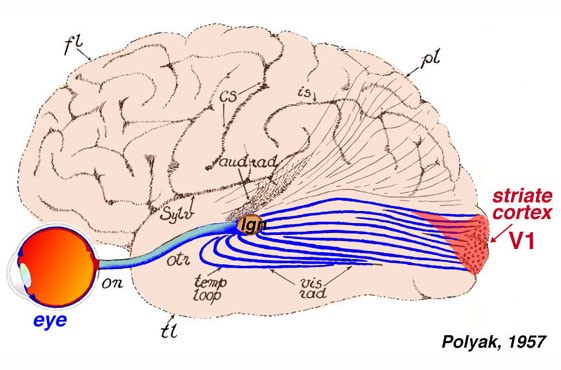
\includegraphics[width=0.25
             \textwidth]{presentation/figures-models/v1.jpg}
                \caption{Visual input goes from the eye to primary visual cortex (V1). Adapted from Polyak (1957).}
            \end{figure} 
            
The central question we will be investigating in this project is the following: how is the structure of artificial neural networks (ANNs) related to that of neurobiological networks in the primary visual cortex? This remains an open question.
    
\par One challenge of comparing the neural network structures is that the neural responses (from both V1 and ANNs) are usually encoded in high-dimensional representation.  Our approach to this question is to infer a neural manifold using dimensionality reduction methods on the neural responses. Informally, the neural manifold shows the clusters of neurons grouped by their firing patterns in response to a given visual stimulus.  This manifold structure implies a functional network (represented by the discrete data graph underlying the continuous manifold) and thus reflects both the neural circuit connections and the neuron’s role in those circuits. 

\par We then compare the neural manifolds in biological and artificial neural networks. For the latter, we will be investigating Convolutinoal Neural Networks (CNNs), Recurrent Neural Networks (RNNs) and the latest Transformer and Perceiver networks. By comparing the manifold structures of biological and artificial neural networks we can make precise inferences about similarities and differences in their respective functional circuits.
  
\par The significance of achieving the goals outlined above is twofold. First, there is significant interest in comparing the structure of artificial and biological neural networks. Artificial neural networks have proved capable of many computer vision tasks at a level competitive to biological systems. However, whether artificial and biological neural networks have the same functional circuit remains an open question. (\cite{Gwilliams221630}) 

\par Second, modeling the visual system is an important task. In the field of neuroscience, despite decades of research, we have not fully understood the science behind visual perception. In the field of AI, more sophisticated models of the visual system could inspire new computational algorithms in solving increasingly demanding computer vision tasks. In fact, research in computer vision has taken many inspirations from neuroscience. In LeCun, Bengio, \& Hinton's seminal work on deep learning (\cite{lecun_deep_2015}), they stated that ``ConvNets have their roots in the Neocognitron," which was one of the earliest computational models of the visual system. 

\section{Historical context}

\par The earliest efforts in modeling the visual system began with Hubel and Wiesel's hierarchy model in the 1960s. Sine then, numerous alternative models were proposed, such as the parallel models and recurrent models, all of which aimed to more accurately reflect the actual neural connectivity in the visual system. 

\subsection{Hierarchy Models}
\par Hubel and Wiesel's hierarchy model (\cite{hubel_receptive_1962}) was the first seminal work on modeling the visual system, which classified the neurons in the primary visual cortex (V1) into simple cells and complex cells. The essential difference between the simple cells and complex cells is that the responses of simple cells are modulated by the spatial phase of a sine grating, whereas the responses of complex cells are largely phase invariant. In other words, as we progress from simple cells to complex cells, the neurons become selective for increasingly complex stimuli and at the same time become more tolerant to the exact position within their receptive fields. 

\par Based on this, a natural way to construct complex cells is to group responses from simple cells with the same orientation preference, but with different phase preferences.

\par This idea directly inspired the Neocognitron model (\cite{fukushima_neocognitron_1980}). In the Neocognitron model, simple cells (termed as ``S-cells" in the original paper) are tuned to simple stimuli at the convolution layers. Their outputs are then combined at the pooling layers by taking the maximum or average to form complex cells (termed as ``C-cells" in the original paper). As a result, complex cells are tuned to more complex stimuli. 

\par The Neocognitron model was among a myriad of hierarchical models of the visual system. It went on to inspire the Convolutional Neural Networks (CNNs), a class of artificial neural networks that has become dominant in various computer vision tasks. (\cite{yamashita_convolutional_2018})

\par The figure below shows a systematic illustration of the general idea behind the hierarchical models:
\begin{figure}[H]
\centering
    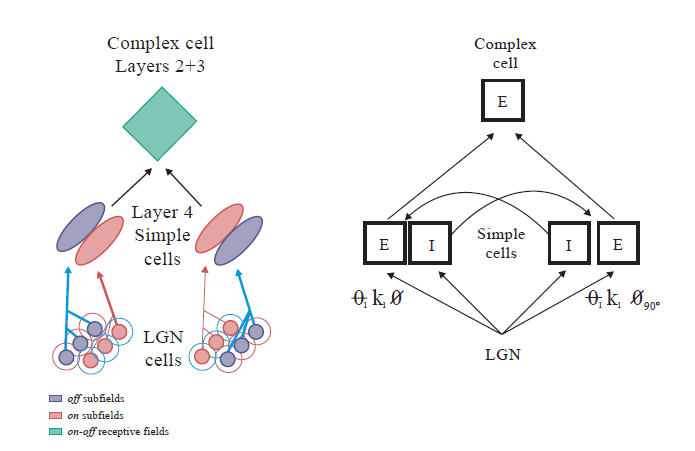
\includegraphics[width=10cm]{figures/models/hierarchical-models.png}
     \caption{Illustration of the hierarchical models (\cite{martinez_complex_2003})}
\end{figure}

\par The possible advantages of hierarchical models are as follows:
\begin{itemize}
    \item If a visual recognition task can be decomposed into low-complexity learning tasks for each layer of a hierarchical learning machine, then each layer may require only a small number of training examples (\cite{poggio2003mathematics}).
    \item The lowest levels of the hierarchy may represent a dictionary of features that can be shared across multiple classification tasks (\cite{geman1999hierarchy}), thus increasing efficiency.
\end{itemize}

\par There are also some known limitations of hierarchical models:
\begin{itemize}
    \item Hierarchical models assume that the computations at each successive stage being largely feed-forward (\cite{riesenhuber1999hierarchical}, \cite{dicarlo2012does}). This is limited because back-projections are also likely to be a key part of the visual system. 
    \item There remains a very broad distribution of tuning and receptive field sizes in all areas of the visual hierarchy. Hence, the anatomical hierarchy should be taken as an idealization and cannot be taken as a strict flowchart of visual information (\cite{hegde2007reappraising}). 
    % \par One particularly interesting piece of evidence: a close comparison of shape representation between V1, V2 and V4 also demonstrated a complex pattern of shape selectivity with significant deviation from strict hierarchical organization with some cells in V1 exhibiting more complex tuning than some cells in V4 (\cite{hegde2007reappraising}).
\end{itemize}

\subsection{Alternative Models}
\par Since Hubel and Wiesel proposed the classification of simple cells and complex cells, many other hierarchical models have been proposed for a more realistic representation for the cortical circuitry. Furthermore, new experimental and computational evidence provided serious alternatives to this hierarchical model, including parallel models and recurrent models (\cite{martinez_complex_2003}). There are still many controversies and debates over which models best capture neural mechanisms of the visual system.

\subsubsection{Parallel Models}
\par The first strong evidence against the hierarchical model was the discovery that some complex cells, like simple cells, receive monosynaptic input from the thalamus (\cite{hoffmann1972relay}). Based on this discovery, Hoffman and Stone proposed that both cell types, simple and complex, were generated in parallel by separate thalamocortical pathways, as shown in diagram A in Figure \ref{fig:parallel-models}. 
\begin{figure}[H]
\centering
    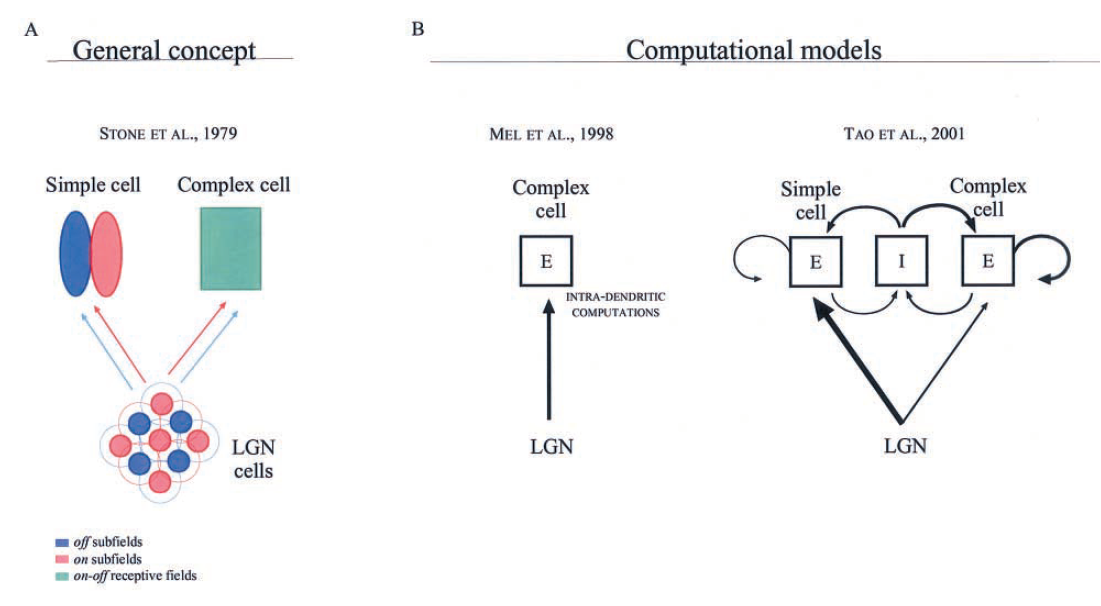
\includegraphics[width=10cm]{figures/models/parallel-models.png}
     \caption{Illustration of the parallel models (\cite{martinez_complex_2003})}
     \label{fig:parallel-models}
\end{figure}

\par Simple cells and complex cells are far from being two parallel cortical pathways in the same way that X and Y cells are parallel thalamic pathways. However, the idea that some complex receptive fields can be generated at
least in part by direct thalamic inputs is likely to be correct. (\cite{martinez_complex_2003})

\subsubsection{Recurrent Models}
\par Recurrent models changed the focus of attention from single cells to networks of cortical connections. (\cite{martinez_complex_2003}) An illustration for recurrent models are shown in Figure \ref{fig:recurrent-models}.

\begin{figure}[H]
\centering
    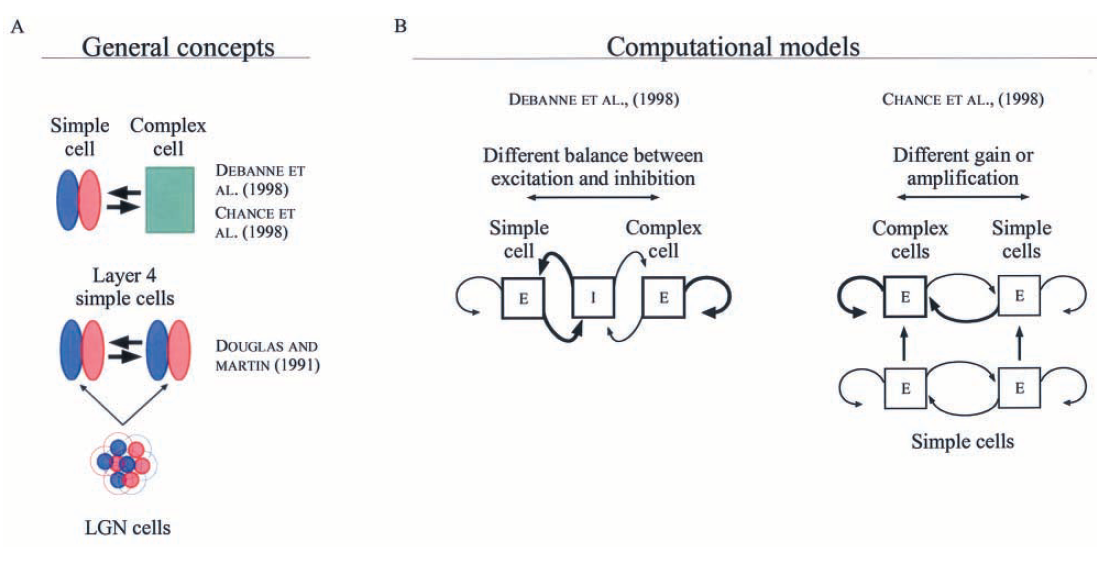
\includegraphics[width=10cm]{figures/models/recurrent-models.png}
     \caption{Illustration of the recurrent models (\cite{martinez_complex_2003})}
     \label{fig:recurrent-models}
\end{figure}

\section{Related works on geometric and topological approach to neural networks}
Throughout the historical progress in neuroscience, there have been numerous efforts to apply geometric and topological methods from related fields in mathematics and computer science, including computational geometry, differential geometry, spectral graph theory, and algebraic topology, among many others. Recently, studying the structure of neural population response with high-dimensional neural spiking data has become a commonly used technique in studying the structure of brain cortices. The high-dimensional nature of neural spiking data have thus motivated various dimensionality reduction methods, both linear and non-linear. 

The paper (\cite{chung_neural_2021}) provided a comprehensive review of the recent studies that have applied geometric and topological methods to discover the properties of neural population geometry. 
% \cite{chung_classification_2018} proposed the ``object manifold" which

The authors of (\cite{gallego_neural_2017}) were the first to propose the concept of ``neural modes," which are specific patterns of correlated neural activity that span the neural manifolds. They thus proposed a generative model of individual neuronal activity based on the activation of neural modes. The parameters of such model can be obtained using dimensionality reduction methods. \cite{williams_unsupervised_2018} used linear dimensionality reduction method of tensor canonical polyadic (CP) decomposition to discover low-dimensional neural dynamics by extracting three ``tensor factors," which are interconnected, low-dimensional descriptions of neural data.

The first work that applied topological methods in neuroscience is (\cite{singh_top_v1_2008}). The authors applied computational topology to analyze neural population activity in the primary visual cortex and concluded that the topological structure of neural population activity is align with the topological structure of a $2$-sphere both when the cortex is spontaneously active and when evoked by natural images.

Following that, there have been many applications of persistent homology in studying the topological structure of neural population activity across different systems. A notable application is (\cite{chaudhuri_intrinsic_2019}), where the authors applied persistent homology to study the the neural population activity from the post-subiculum and anterodorsal thalamus. They showed that the head direction of mice can be decoded from a one-dimensional ring structure. A recent addition to this line of work was (\cite{beshkov_geodesic-based_2021}). The authors of this paper showed that when using the geodesic distance instead of the Euclidean distance, persistent homology method was able to successfully identify highly non-linear features. They then provided an application using the Neuropixels dataset recorded in mouse visual cortex after stimulation with drifting gratings.

\section{Organization of the report}

\par The current chapter outlined the goals and significance of this project, historical background of the research question, and related works. Chapter 2 will give an overview of the methodology and Chapters 3 and 4 will address the different parts of the methodology in greater details. Chapter 5 and 6 will present the implementation details on the experiments for biological and artificial neural networks, respectively. Chapter 7 is an extension of the method to study the topological features of the manifold structure. Chapter 8 will summarize the tasks and results completed during this semester and provide a blueprint for the next steps.
\chapter{Overview of Methodology} 
\label{chapter-outline}

\section{Main objective}

The main objective of our project is to study the manifold structure of biological and artificial neural networks. This objective is equivalent to generating the underlying neural manifolds from data that are obtained from biological and artificial neural networks respectively. In what follows, we will give an overview of the methodology according to the following quesions:
\begin{itemize}
    \item What is a neural manifold?
    \item How to generate the neural manifold?
    \item What can we analyze from the neural manifold?
\end{itemize}


\section{What is a neural manifold?}
Before explaining the idea behind ``neural manifold" in the context of neuroscience, we first introduce the general concept of a manifold as a mathematical object.

\begin{defn}[Homeomorphism]
A continuous map $f: X \to Y$ be a function between topological spaces $X$ and $Y$. If $f$ is bijective, then the inverse $f^{-1}$ exists. If both $f$ and $f^{-1}$ are continuous, then $f$ is a \underline{homeomorphism}. The two topological spaces, $X$ and $Y$, are said to be \underline{homeomorphic} if there exists a homeomorphism between $X$ and $Y$. 
\end{defn}
    \begin{defn}[Manifold]
   In brief, a \underline{real $n$-dimensional manifold} is a topological space $\mathcal{M}$ for which every point $x\in\mathcal{M}$ has a neighborhood homeomorphic to Euclidean space $\RR^n$.
    \end{defn}
   \begin{figure}[H]
      \centering
     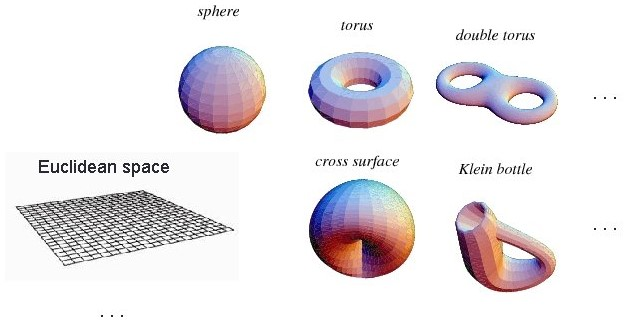
\includegraphics[width=0.4\textwidth]{presentation/manifold.jpg}
     \caption{Examples of $2$-dimensional manifolds.}
    \end{figure} 
            
Our approach to study the neural population response via the neural manifold is based on the premise of ``the Manifold Hypothesis," which states that real-world high-dimensional data lie on a low-dimensional manifold embedded within the high-dimensional space. (\cite{deepai_2019}) The original representation of data has a large degree of freedom, that is, the number of variables that are really necessary to describe the data is much smaller than the number of variables in the original representation. 

% We can illustrate this hypothesis with image data: an image is high-dimensional since the number of dimensions of an image equals the number of pixels. Each image can be reparameterized with much smaller number of variables after applying appropriate feature extraction algorithms. 

% main idea behind manifold learning:
In the context of neuroscience, neural spiking data are usually high-dimensional due to the kind of data representation (the peristimulus, or PSTH, diagrams) determined by the lab instrument. However, it has been shown that the neural connections constrain the possible patterns of neural population activity (\cite{okun_diverse_2015}, \cite{sadtler_neural_2014}, \cite{tsodyks_attractor_1999}) and that the possible patterns are confined to a low-dimensional manifold (\cite{stopfer_intensity_2003},  \cite{yu_gaussian-process_2009}) spanned by a few independent patterns that are called ``neural modes." (\cite{gallego_neural_2017})

We call this underlying low-dimensional manifold the ``\textbf{neural manifold}." The distance between a pair of points on the neural manifold indicate how similar their firing patterns are in response to a given visual stimulus. Intuitively we can understand the neural manifold as a collection of clusters of neurons grouped by their firing patterns in response to a given visual stimulus. Figure \ref{fig:neural-manifold-eg} shows an example of a neural manifold generated from neural spiking data. 

 
      \begin{figure}[H]
        \centering
      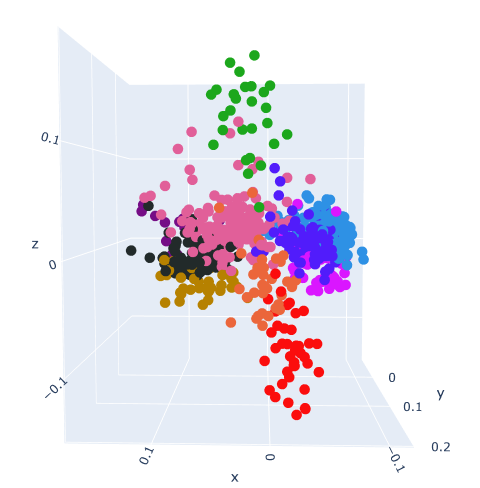
\includegraphics[width=0.8\textwidth]{figures/embeddings/embedding-lab.png}
      \caption{Visualize an example of a neural manifold generated from neural spiking data.}
      \label{fig:neural-manifold-eg}
            \end{figure} 
            
\section{How to generate the neural manifold?}
The task of generating the neural manifold is equivalent to learning\footnote{``Learning" here refers to unsupervised learning, which is a class of approaches in machine learning that discover meaningful features without training data.} the low-dimensional manifold underlying the original high-dimensional neural spiking data, which amounts to a dimensionality reduction task. In our project, we use both the linear dimensionality reduction method tensor canonical polyadic (CP) decomposition and the non-linear dimensionality reduction method diffusion map. The theoretical preliminaries for these two methods will be explained in full details in the next two chapters.

\section{What can we analyze from the neural manifold?}

We can directly compare the low-dimensional neural manifold for the biological neural networks with that for the artificial neural networks. The neural manifolds implies a functional network. The functional network is represented by the discrete data graph underlying the continuous manifold and thus reflects both the neural circuit connections and the neuron’s role in the circuit. We can thus make precise inferences about the similarities and differences between the particular biological and artificial neural networks in terms of their respective functional circuit, which is what we set out to compare. 


We can further extend this comparison to the \textit{topological} properties of the neural manifolds by extracting the topological features via persistent homology and quantifying the topological similarities using appropriate distance metric between the topological features. In our study, we have chosen the commonly used $p$-Wasserstein distance to quantify the pairwise similarities between the topological features of the neural manifolds given different stimuli. 

The following flowchart showed a schematic summary of the methodology of the project.

\bigskip

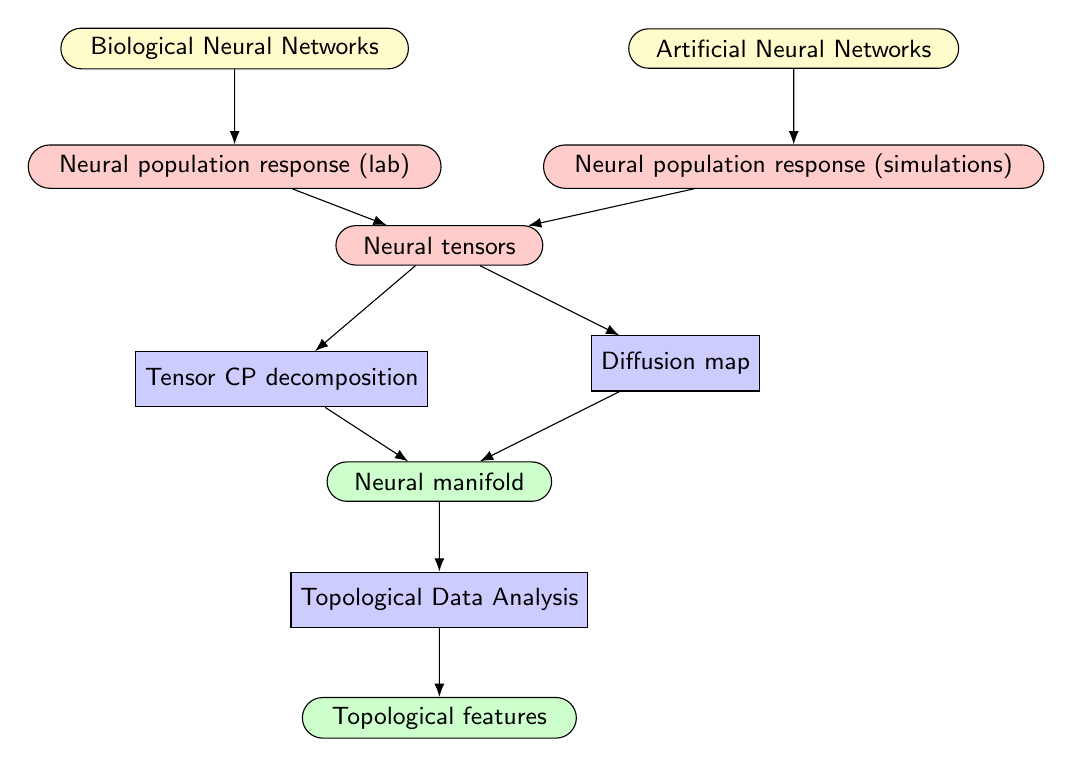
\begin{tikzpicture}[font={\sf \small}]
 \def\smbwd{2cm}
  \node (BNN) at (-3.6,0.5) [draw, terminal, minimum width=\smbwd,  fill=yellow!20, minimum height=0.5cm] {Biological Neural Networks}; 
  \node (ANN) at (3.5,0.5) [draw, terminal, minimum width=\smbwd,  fill=yellow!20, minimum height=0.5cm] {Artificial Neural Networks}; 
  %------------
  \node (experimental) at (-3.6,-1) [draw, terminal, minimum width=\smbwd,  fill=red!20, minimum height=0.5cm]{Neural population response (lab)};
  \node (artificial) at (3.5,-1)[draw, terminal,minimum width=\smbwd,  fill=red!20, minimum height=0.5cm]{Neural population response (simulations)};
  %------------
  \node (tensors) at (-1,-2) [draw, terminal, minimum width=\smbwd,  fill=red!20, minimum height=0.5cm] {Neural tensors}; 
  %------------
  
  \node (TCA) at (-3,-3.7) [draw, process, minimum width=\smbwd, fill=blue!20, minimum height=0.7cm] {Tensor CP decomposition};
  \node (diffusion) at (2,-3.5) [draw, process, minimum width=\smbwd, fill=blue!20, minimum height=0.7cm] {Diffusion map};
  %------------
  
  \node (manifolds) at (-1,-5) [draw, terminal, minimum width=\smbwd,  fill=green!20, minimum height=0.5cm] {Neural manifold};
  
  \node (TDA) at (-1,-6.5) [draw, process, minimum width=\smbwd, fill=blue!20, minimum height=0.7cm] {Topological Data Analysis};
   
 \node (topology) at (-1,-8) [draw, terminal, minimum width=\smbwd,  fill=green!20, minimum height=0.5cm] {Topological features};
 
  %------------
 
 \path [line](BNN) -- (experimental);
 \path [line](ANN) -- (artificial);
 \path [line](tensors) -- (TCA);
 \path [line](tensors) -- (diffusion);
 \path [line](experimental) -- (tensors) ;
 \path [line] (artificial) -- (tensors) ;
 \path [line](diffusion) -- (manifolds);
 \path [line](TCA) -- (manifolds);
  \path [line](manifolds) -- (TDA);
  \path [line](TDA) -- (topology);
 \end{tikzpicture}
 
 % 

% Consider a set of $N$ neurons responding to a specific sensory signal associated with an object. The neural population response to that stimulus is a vector in $\mathbb{R}^N$. 

% We model a set of $P$ manifolds corresponding to $P$ objects.
% Each manifold $M_\mu$ for $\mu 1, \dots, P$ consists of a compact
% subset of an affine subspace of $\mathbb{R}^N$ with affine dimension $D$ with $D < N$. A point on the manifold $x_\mu \in M_\mu$ can be parametrized as
% \begin{align}
%     \xx^\mu(\vec{S}) = \sum_{i = 1}^{D+1} S_i \uu^\mu_i
% \end{align}
% (Notations adapted from \cite{chung_classification_2018})
\chapter{Preliminaries on Tensor CP decomposition } 
\label{chapter-linear} 

This chapter explains in detail the linear dimensionality reduction method used in this project, tensor canonical polyadic (CP) decomposition, a higher-order generalization of principal component analysis (PCA).

\section{PCA}
Principal component analysis (PCA) is the simplest matrix decomposition model. The PCA model can be formulated as an optimization problem. Given a $N$-by-$M$ matrix $\mathbf{X}$ with $N$ variables and $M$ features, we can approximate $\mathbf{X}$ with the product of two orthogonal rank-one matrices:
\begin{align}
    \mathbf{X} \approx \mathbf{U}\mathbf{V}^T = \sum_{r=1}^R u_r \circ v_r,
\end{align}
where $\circ$ denotes the outer product operator. The equivalent element-wise formulation of the PCA model is
\begin{align}
\label{pca}
    x_{i j} \approx \sum^R_{r = 1} u_i^r v_j^r.
\end{align}
With PCA, the dimensionality of the original matrix can be reduced from from $N$-by-$M$ to $N$-by-$R$. This can be illustrated with the diagram below
\begin{figure}[H]
    \centering
        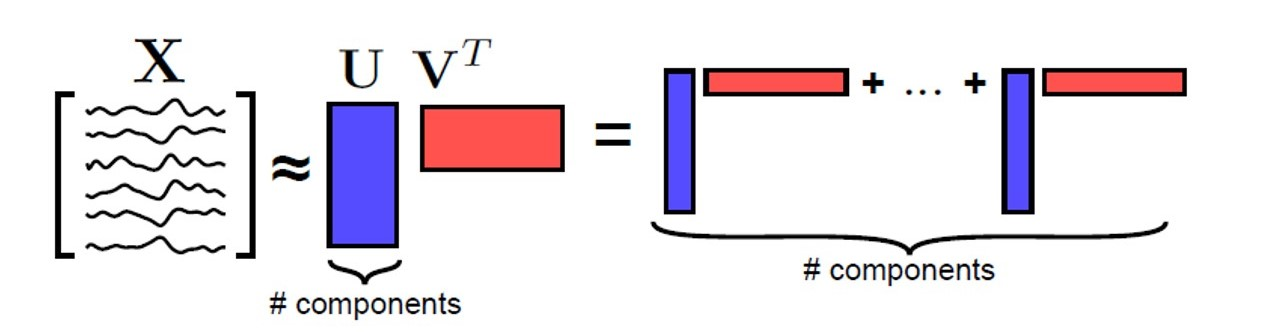
\includegraphics[width=0.7\textwidth]{figures/linear/pca.jpg}
        \caption{Illustration for PCA. (Adapted from (\cite{williams_unsupervised_2018}))}
    \end{figure} 

\begin{itemize}
    \item maximize variance:
\begin{maxi}|l|
  {\mathbf{V}}{\|\mathbf{X}\mathbf{V}\mathbf{V}^T\|_F^2}{}{}
  \addConstraint{\mathbf{V}\text{ orthonormal}}
 \end{maxi}
 \item minimize residuals:
 \begin{mini}|l|
  {\mathbf{U},\mathbf{V}}{\|\mathbf{X} - \mathbf{U}\mathbf{V}^T\|_F^2}{}{}
  \addConstraint{\mathbf{U,V}\text{ orthogonal}}
 \end{mini}
 \begin{rmk}
 Note that without the constraint of $\mathbf{U},\mathbf{V}$ being orthogonal, PCA has infinite number of solutions since
 $\mathbf{U}\mathbf{V}^T = \mathbf{U}F^{-1} F\mathbf{V}^T = \mathbf{U}^\prime \mathbf{V}^{\prime T}.$
 \end{rmk}
\end{itemize}

\par When the data has a non-negative constraint, non-negative matrix factorization (NMF) is used. In NMF, the second part of the optimization becomes the following instead:
 \begin{mini}|l|
  {\mathbf{U},\mathbf{V}}{\|\mathbf{X} - \mathbf{U}\mathbf{V}^T\|_F^2}{}{}
  \addConstraint{\mathbf{U}\geq 0, \mathbf{V} \geq 0.}
 \end{mini}

\section{Higher-order generalization of PCA: tensor CP decomposition}
The main references for this section are  (\cite{williams_unsupervised_2018}),
(\cite{kolda_tensor_2009}), and (\cite{hong_generalized_2020}).

Tensor  canonical polyadic (CP) decomposition generalizes PCA from matrices to higher-order tensors.
\begin{defn}[Tensor norm]
The \underline{norm of tensor} $\mathcal{X} \in \RR^{I_1 \times I_2\times\cdots I_N}$ is
\begin{align}
    \norm{\mathcal{X}} = \sqrt{\sum_{i_1 = 1}^{I_1}\sum_{i_2 = 1}^{I_2}\cdots \sum_{i_N = 1}^{I_N} x_{i_1 i_2 \dots i_N}^2 }.
\end{align}
\end{defn}

\begin{defn}[Rank-one tensors]
An $N$-way tensor $\mathcal{X} \in \RR^{I_1 \times I_2\times\cdots I_N}$ is \underline{rank-one} if it can be written as the outer product of $N$ vectors, that is,
\begin{align}
    \mathcal{X} = \vec{a}^{(1)}\circ \vec{a}^{(2)} \circ \cdots \circ \vec{a}^{(N)}
\end{align}
\end{defn}

Analogous to PCA, tensor CP decomposition aims to approximate the original tensor by a sum of rank-one tensors, each of which can then be written as the outer product of $N$ vectors. Given a $3$-way tensor $\mathcal{X} \in \RR^{I\times J\times K}$, the tensor CP decomposition model is formulated as
\begin{align}
    \mathcal{X} \approx [\![ \mathbf{A}, \mathbf{B}, \mathbf{C} ]\!] = \sum_{r=1}^R a_r \circ b_r \circ c_r,
\end{align}
where $R$ is the number of components and $a_r \in \RR^I, b_r \in \RR^J, c_r \in \RR^K$ for $r = 1,\dots, R.$ The element-wise formulation analogous to \ref{pca} is 
\begin{align}
    x_{i j k} \approx \sum_{r=1}^R a_{i r} b_{j r} c_{k r}
\end{align}
for $i = 1,\dots, I, j = 1,\dots, J, k = 1,\dots,K.$

With tensor CP decomposition, we obtain the tensor factors which are analogous to the principle components. This can be illustrated with the diagram below
\begin{figure}[H]
    \centering
        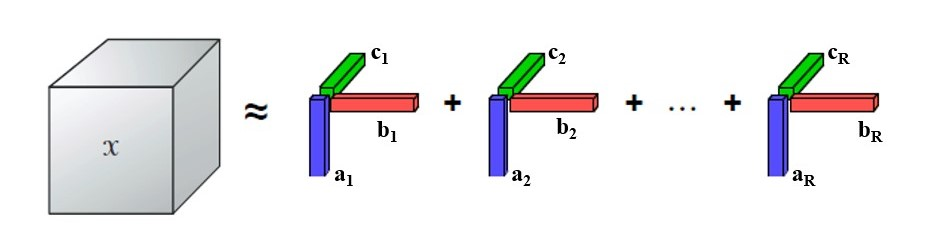
\includegraphics[width=0.7\textwidth]{figures/linear/tca.jpg}
        \caption{Illustration for tensor CP decomposition. (Adapted from (\cite{williams_unsupervised_2018})}
    \end{figure} 
    
The alternating least squares (ALS) method is one of the most common algorithms to compute a tensor CP decomposition with $R$ components. The steps of the ALS are summarized as follows: 
\begin{enumerate}
    \item fix  $\mathbf{B}$ and  $\mathbf{C}$ to solve for $\mathbf{A}$: 
     \begin{equation}
       \min_{\mathbf{A}} \sum_{i j k}\left(x_{i j k} - \sum_l a_{i l} b_{j l} c_{k l}\right)^2
     \end{equation}
    \item fix $\mathbf{A}$ and  $\mathbf{C}$ to solve for  $\mathbf{B}$:
  \begin{align}
       \min_{\mathbf{B}} \sum_{i j k}\left(x_{i j k} - \sum_l a_{i l}  b_{j l} c_{k l}\right)^2
     \end{align}
 \item fix $\mathbf{A}$ and  $\mathbf{B}$ to solve for $\mathbf{C}$: 
 \begin{align}
       \min_{\mathbf{C}} \sum_{i j k}\left(x_{i j k} - \sum_l a_{i l}  b_{j l} c_{k l}\right)^2
     \end{align}
\end{enumerate} 
and repeat the above steps until some convergence criterion is satisfied. 

\section{Demonstrate tensor CP decomposition by using the face image dataset}
As an intuitive demonstration for the tensor CP decomposition method, we apply tensor CP decomposition on face image data with 1000 face images, with each image having dimension $96$-by-$96$. Thus, the face image data are encoded in a $3$-way tensor of dimension $1000$-by-$32$-by-$32$. Using tensor CP decomposition, we obtain the first $5$ tensor components, which intuitively represent the prominent facial features in the face images: 
\begin{figure}[H]
    \centering
        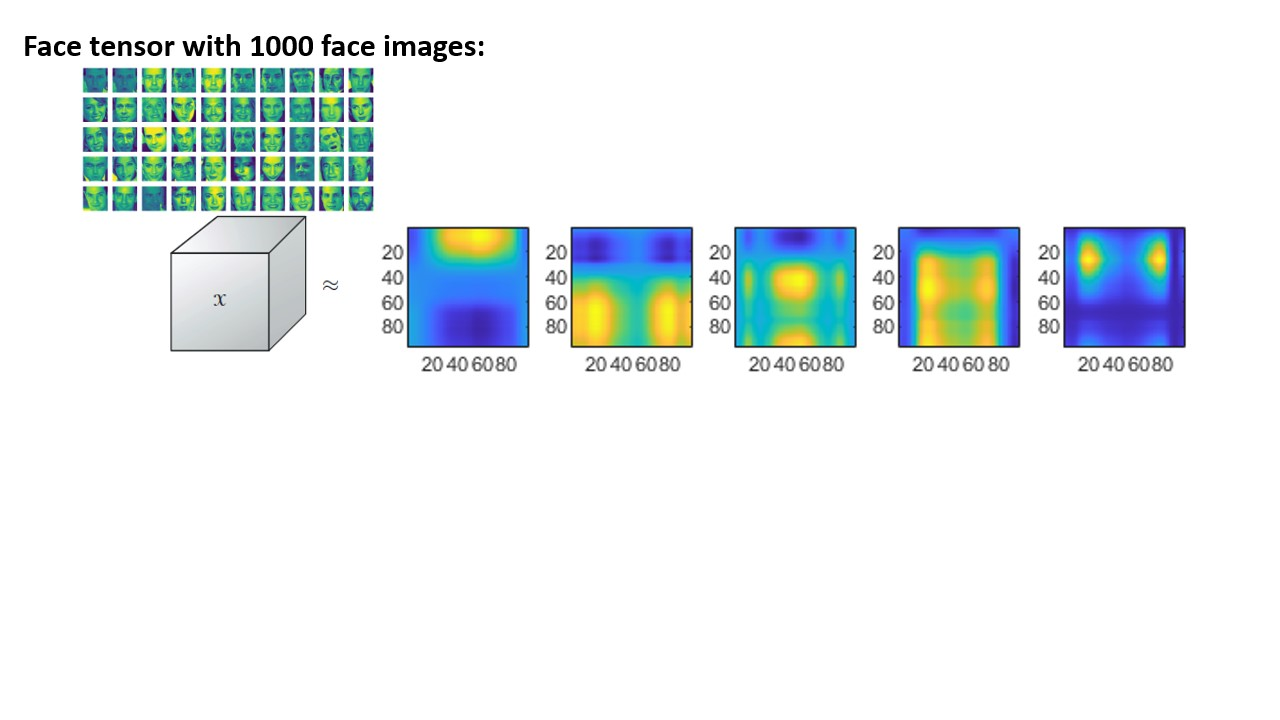
\includegraphics[width=0.7\textwidth]{presentation/Slide2.jpg}
        \caption{First 5 tensor factors for face image data.}
    \end{figure}

By projecting the data onto the first few principal components and apply the $k$-means clustering method, we obtain the following clusters grouped by similar face images: 
\begin{figure}[H]
    \centering
    \begin{subfigure}[b]{0.45\textwidth}
        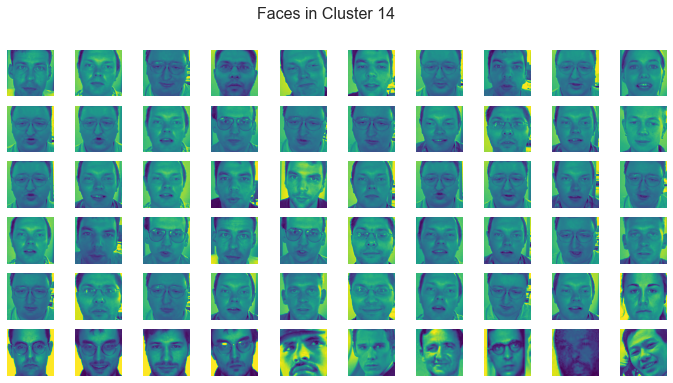
\includegraphics[width=\textwidth]{presentation/figures-face-results/face14.png}
    \end{subfigure}
    \hfill 
    \begin{subfigure}[b]{0.45\textwidth}
        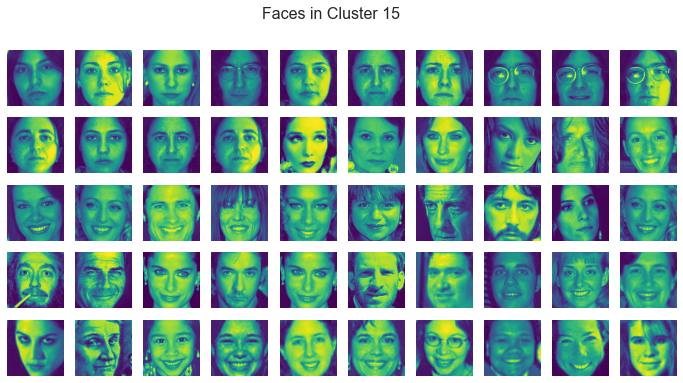
\includegraphics[width=\textwidth]{presentation/figures-face-results/face15.png}
    \end{subfigure}
    \hfill
    \begin{subfigure}[b]{0.45\textwidth}
        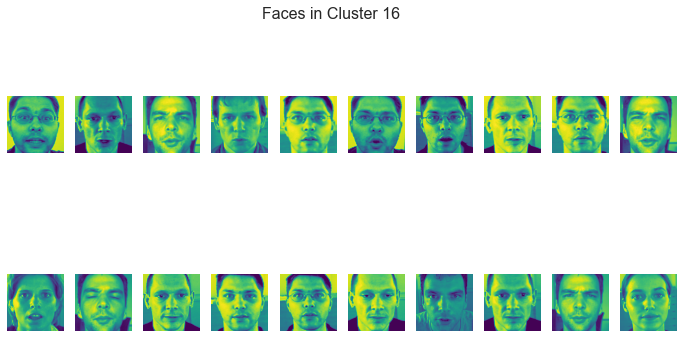
\includegraphics[width=\textwidth]{presentation/figures-face-results/face16.png}
    \end{subfigure}
    \hfill
    \begin{subfigure}[b]{0.45\textwidth}
        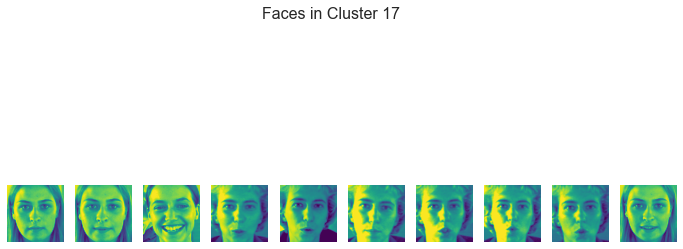
\includegraphics[width=\textwidth]{presentation/figures-face-results/face17.png}
    \end{subfigure}
    \caption{Some arbitrary clusters showing the results of tensor CP decomposition for face data.}
    \end{figure} 
    
\section{Remarks on linear dimensionality reduction}
Linear dimensionality reduction techniques work well when the data lie near a linear subspace of high-dimensional space. They do not work well when the data lie near a non-linear manifold embedded in the high-dimensional space. (\cite{fefferman_testing_2016}) Due to this reason, we introduce the non-linear dimensionality reduction technique of diffusion map in the next chapter. 
\chapter{Preliminaries on Diffusion Map} 
\label{chapter-nonlinear} 

In this chapter we introduce the non-linear dimensionality reduction method of diffusion map. The main references for this section are (\cite{coifman_geometric_2005}),   (\cite{coifman_diffusion_2006}) and (\cite{stanley_geometric_2020}). We will now outline the steps in the diffusion map algorithm.
\begin{enumerate}
\item Discretize the underlying manifold as a weighted graph.
\begin{defn}[Discretization of a manifold]

Given $X = \{x_1, x_2,\dots, x_n\}$, a set of data sampled from a Riemannian manifold $\mathcal{M}$, we can construct the discretization of $\mathcal{M}$ as as a weighted, undirected graph, $\mathcal{G}_X = (X, g_\epsilon)$ where $X$ is the set of vertices given by the data and $g_\epsilon$ is a Gaussian kernel function $g_\epsilon: (x_i, x_j) \to [0,\infty]$ defined by the following rule
\begin{align}
    g_\epsilon(x_i,x_j) = \frac{1}{2}\left(\exp{\frac{-\|x_i - x_j\|_2^2}{2\epsilon(x_i)}} + \exp{\frac{-\|x_i - x_j\|_2^2}{2\epsilon(x_j)}}\right), \quad \forall x_i,x_j \in X, 
\end{align}

 where $\epsilon: X \to \RR$ is the the bandwidth function by which the Gaussian kernel is parameterized. 
\end{defn}

Gaussian kernel is only one of the possible kernel functions, but it gives a physically intuitive construction for learning the manifold underlying the data sample because it effectively considers a ball of radius $\epsilon$ around each data point.

The choice of $\epsilon$ determines the radius of neighborhood of $x_i \in X$. $\epsilon$ is application-specific and is usually a global bandwidth, that is, $\epsilon(x_i) = \epsilon(x_j)$ for all $x_i, x_j \in X.$ 

\item Compute the similarity matrix associated with the weighted graph.

Given the weighted graph $\mathcal{G}_X$, we can compute the corresponding similarity matrix. Each entry in the similarity matrix, $W_{i j}$, is the pairwise similarity value between data/vertices $x_i$ and $x_j$ and is taken as the weight of the edge between nodes $x_i$ and $x_i$. 
    \begin{align}
        W_{i j } = \exp\{-\frac{\|x_i - x_j\|^2}{2\sigma^2}\}.
    \end{align}
    
\item Construct a lazy random walk on $\mathcal{G}_X$. 

First, we define random walk on the weighted, undirected graph $\mathcal{G}_X$: 

\begin{defn}[Random walk on graphs]
A \underline{random walk} on $\mathcal{G}_X = (X,g_\epsilon)$ is a process that begins at some vertex $x_i$, and at each time step moves to another vertex $x_j$. Since the graph is weighted, it moves to a neighbor $x_j$ with probability $p(j \mid i)$, proportional to the weight of the corresponding edge, and is defined as follows:
\begin{align}
        p(j\mid i) = \frac{W_{i j}}{\sum_{k} W_{i k}}.
\end{align}
The random walk is \underline{lazy} if we allow $p(i\mid i) > 0$, i.e., the probability of staying at some point $i$ as the time step moves forward is non-zero.
\end{defn}
    
    The probabilities $p(j \mid i)$ can be represented by a Markov matrix $M$, which is essentially the similarity matrix normalized to have row sums equal to $1$:
     \begin{align}
        M = D^{-1} W, \text{where } D_{i i} =\sum_{k}W_{i k}.
    \end{align}
    The probability of reaching node $x_j$ from $x_i$ after $t$ steps is then
    \begin{align}
        p(t,j\mid i) = e_i^T M^t e_j.
    \end{align}

    \item Eigendecomposition of the Markov matrix:
    
    The eigendecomposition of $M$ is derived from the eigendecomposition of $M_s = D^{1/2} M D^{-1/2} = \Omega \Lambda \Omega^T$:
    \begin{align}
        M = D^{-1/2}  \Omega \Lambda \Omega^T D^{-1/2} \coloneqq \Psi \Lambda \Phi^T.
    \end{align}
    
    Note that since $\Psi$ and $\Phi$ are mutually orthogonal, $\Psi$ contains the right eigenvectors, as shown below:
     \begin{align}
        M \Psi =  \Psi \Lambda \Phi^T \Psi = \Psi \Lambda =  \Lambda \Psi.
    \end{align}
    
    The eigendecomposition of $M$ after $t$ steps is then
    \begin{align}
        M = \Psi \Lambda^t \Phi^T.
    \end{align}
    \begin{itemize}
        \item Diffusion coordinate functions are the right eigenvectors of Markov matrix scaled by their corresponding eigenvalues: 
        \begin{align}
            \Upsilon \coloneqq \Psi \Lambda.
        \end{align}
        \item Diffusion distance after $t$ steps is the following:
       \begin{align}
            \| e_i^T  \Upsilon - e_j^T \Upsilon  \|^2 = \sum_{k} (p(t,k\mid i) - p(t,k\mid j))^2 (D_{k k}^{-1}).
       \end{align}
       
       \item Infer geometric properties from the growth of eigenvalues of $M$.
       
       For intuition behind the relation between the growth of eigenvalues and the geometric properties of the underlying manifold that we begin with, we consider the following two extreme situations:
       \begin{enumerate}
           \item If the discretization of the underlying manifold is a disconnected graph (none of the nodes are connected), then:
           \[P = I, \lambda_i = \lambda_j \quad \forall i, j, \]
           which implies a flat spectrum with zero decay rate.
           \item If the discretization of the underlying manifold is a fully connected graph (each of the node is connected to all the rest of the nodes), assuming weights of all edges are $1$, then:
            \[\lambda_1 = 1, \lambda_i = 0 \quad \forall i \neq 1.\]
       \end{enumerate}
    \end{itemize}
\end{enumerate}

\par \textbf{Key ideas of diffusion maps: }
\begin{itemize}
    \item The similarity kernel gives us the \textit{local} geometry. As the time steps move forward, we integrate the local geometry and thus reveal the geometric structures at different scales. 
    \item A cluster from a random walk is a region where the probability of escaping this region is low.
\end{itemize}

\section{Demonstration of the method}
As a demonstration of the diffusion maps method, we apply it on synthetic spiral data and MNIST handwritten digits images data:

\begin{figure}[H]
        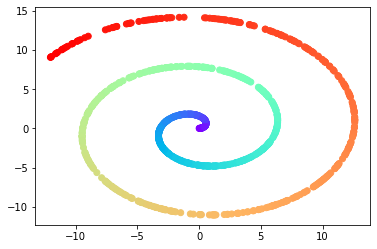
\includegraphics[width=0.6\textwidth]{presentation/spiral.png}
        \caption{Visualising the original spiral data.}
    \end{figure} 
  \begin{figure}[H]         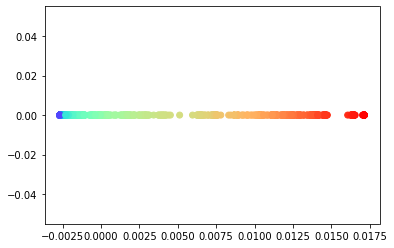
\includegraphics[width=0.6\textwidth]{presentation/spiral-unroll.png}
        \caption{First non-trivial coordinate function.}
        \end{figure} 
\begin{figure}[H]
        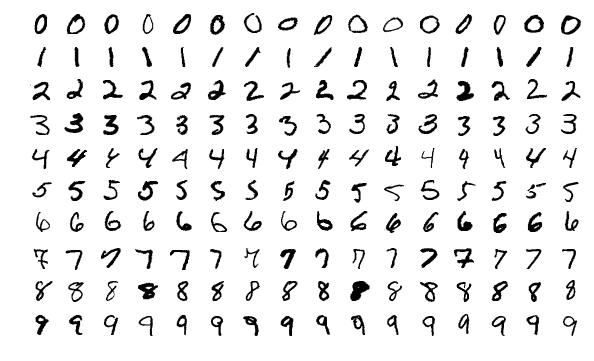
\includegraphics[width=0.4\textwidth]{presentation/mnist-vis.png}
        \caption{Sample data from the MNIST.}
    \end{figure} 
  \begin{figure}[H]
            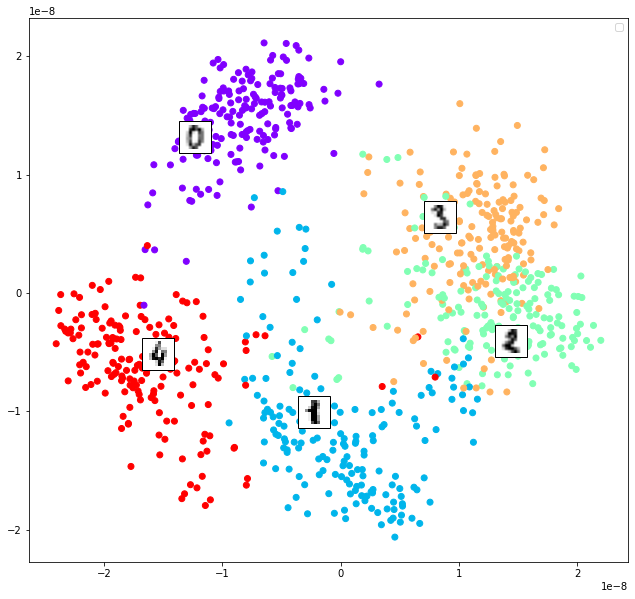
\includegraphics[width=0.6\textwidth]{presentation/mnist.png}
        \caption{First two non-trivial coordinate functions.}    
        \end{figure} 
        
\section{Remarks on non-linear dimensionality reduction}
Setting the right parameters for non-linear dimensionality reduction is very challenging, especially for lab data where sampling errors are prevalent. For this reason, we will be investigating this method in greater details in the second half of the project instead.  
\chapter{Experiments with Biological Neural Tensors} 

\label{chapter-biological} 

\section{Data collection}

The neural spiking data (\cite{dyballa_manifold_2021}) were collected from lab experiments conducted on mice. The experimental setup is shown in the figure below. Visual stimuli of moving artificial gratings of six different types were flashed in front of the mouse. Each visual stimuli were moving in eight directions. Response of neurons in the mouse retina was recorded with electrodes and encoded in peristimulus (PSTH) diagrams. Each PSTH diagram shows the firing rate of one neuron over time for each of the eight directions respectively. Brighter pixels indicate higher firing rates.
\begin{figure}[H]
    \centering
        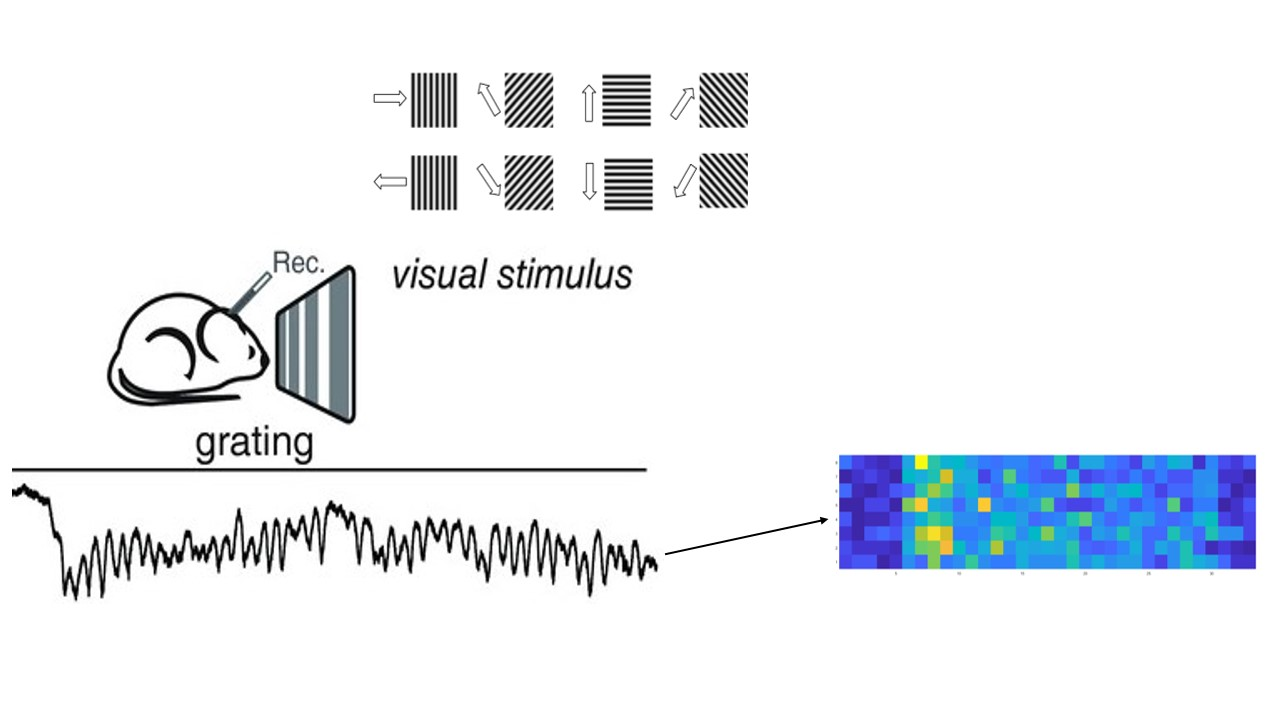
\includegraphics[width=0.6\textwidth]{presentation/Slide5.jpg}
        \caption{Visualising neural data from lab experiments.}
\end{figure}

\par The neural spiking data have $3$ dimensions: the first dimension represents the $698$ neurons, the second dimension represents the six different types of stimuli, and the third dimension represents represents the vectorized PSTH diagrams, each of which has $8\times 33 = 264$ pixels. Due to the number of dimensions, we need to generalize the familiar notion of matrix (which only has two dimensions) to its higher-order analogue, tensors, which we define as follows:

\begin{defn}[Tensors]
    An $N$-way tensor is an element of the tensor product of $N$ vector spaces. 
    
    A $1$-way tensor is a vector, $v = [v_1 \quad v_2 \quad \dots \quad v_n]^T.$ 
    
    A $2$-way tensor is a matrix, 
        $A = \left(\begin{matrix}
        A_{1 1} & A_{1 2} & \dots & A_{1 n}\\
        \vdots & \vdots & \vdots & \vdots \\ 
        A_{m 1} & A_{m 2} & \dots & A_{m n}
        \end{matrix}
        \right).$
    \end{defn}

\begin{defn}[Neural population response]
    Suppose $\mathcal{S}$ is a set of $S$ visual stimuli (e.g., images) $\mathcal{S} = \{s_1, s_2,\dots, s_S\}$, each moving over a time interval of $T$ in $d$ directions. The \underline{neural population response} of a set of $N$ neurons to a stimulus $m_i$ over time is $\mathcal{N} = \{\vec{n}_1, \vec{n}_2, \dots, \vec{n}_N\},$ where $\vec{n}_i \in \mathbb{R}^{dT}$. 
\end{defn}
\begin{defn}[Neural tensors]
    Each \underline{neural tensor} encodes the neural population response of a set of neurons to a set of moving visual stimulus over the time and directions of the movement. It is thus a $3$-way tensor of dimension $N$-by-$S$-by-$dT$.
\end{defn}

\section{Applying tensor CP decomposition}
To implement the tensor CP decomposition, we used the software, Tensor Toolbox for MATLAB. (\cite{tensortoolbox}) Our code is available in the GitHub repository\footnote{https://github.com/zhang-liu-official/capstone-liu-2022} for this project. After obtaining the tensor factors from tensor CP decomposition, we used PCA to project data onto a lower-dimensional linear subspace and k-means to label the clusters by distances in the lower-dimensional linear subspace. 

We can visualize the first five tensor factors from biological neural tensor:
    \begin{figure}[H]
        \centering
            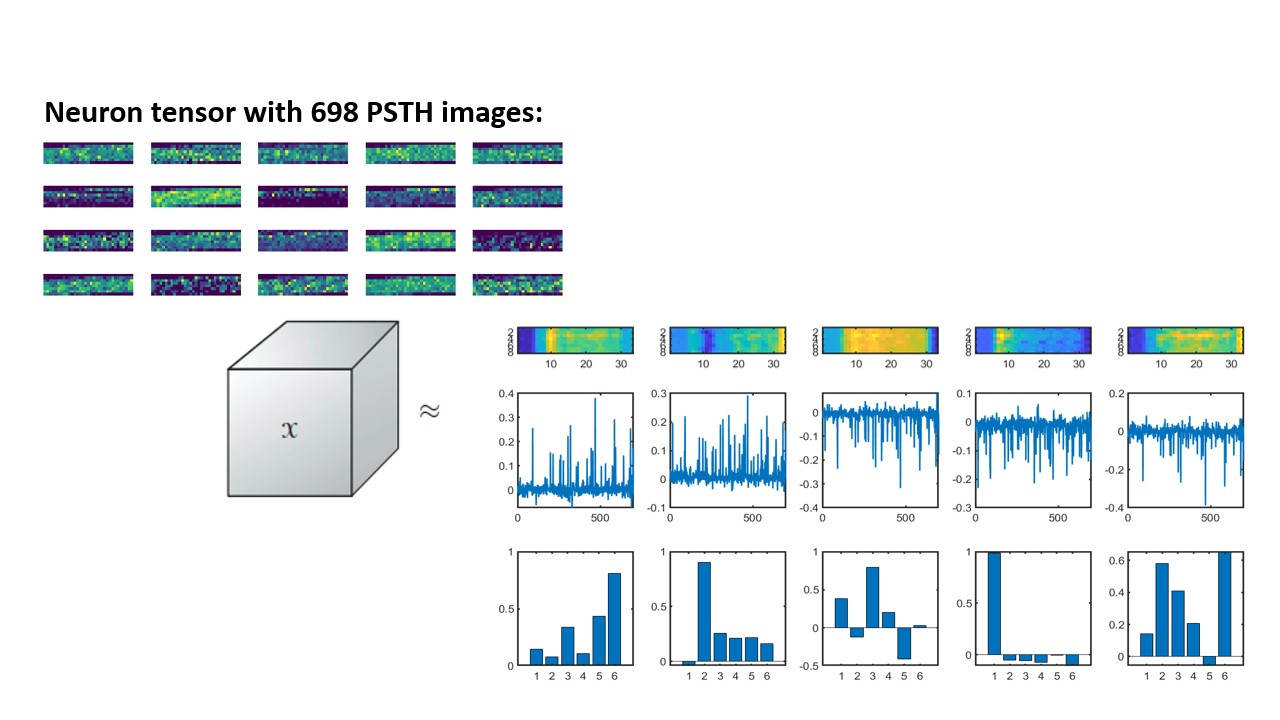
\includegraphics[width=\textwidth]{presentation/Slide3.jpg}
            \caption{First 5 tensor factors for neural data.}
        \end{figure} 

The neural manifold generated from the neural tensor shows the clusters of neurons grouped by their firing patterns encoded in the PSTH diagrams:
    \begin{figure}[H]
        \centering
            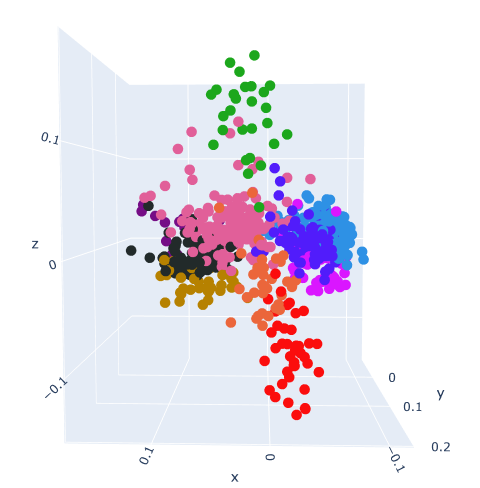
\includegraphics[width=\textwidth]{figures/embeddings/embedding-lab.png}
            \caption{Neural manifolds: clusters of neurons grouped by firing patterns, each point represent a neuron.}
        \end{figure} 

We can plot the PSTH diagrams associated with some points inside the neural manifold, where each point represents a neuron. 

      \begin{figure}[H]
            \centering
            \begin{subfigure}[b]{\textwidth}
                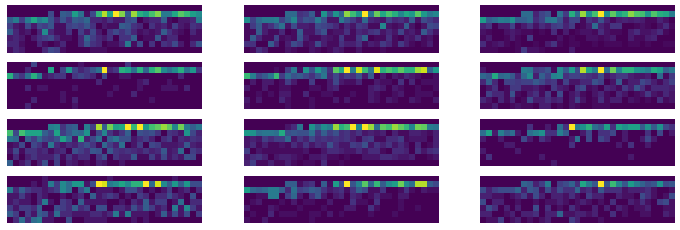
\includegraphics[width=0.95\textwidth]{presentation/figures-retina-results/cluster20.png}
                \caption{PSTH diagrams showing responses of neurons in an arbitrary cluster to stimulus type 1.}
            \end{subfigure}
            \vfill 
            \begin{subfigure}[b]{\textwidth}
                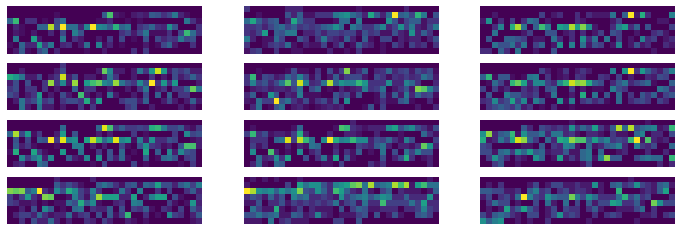
\includegraphics[width=0.95\textwidth]{presentation/figures-retina-results/cluster10.png}
                \caption{PSTH diagrams showing responses of neurons in another cluster to stimulus type 1.}
            \end{subfigure}
            \end{figure} 


\section{Applying diffusion map}
Recall that the neural spiking data set used in this project is represented by a $3$-way tensor of dimension $698$-by-$6$-by-$264$. The three dimensions represent neurons, stimuli, and firing patterns (PSTH diagram) respectively. With this neural spiking data set, we can create six point clouds, each corresponds to the neural population response towards one type of stimuli, which we denote as $X_1, X_2, \dots,X_6$. Each of the point cloud $X_i$ is thus represented by a matrix of dimension $698$-by-$264$, giving us a point cloud of $698$ points in $\RR^{264}$. 

We used the pydiffmap package (\cite{eastman_pydiffmap_2017}). In our implementation, we reduced the dimensionaltity of each point cloud from the space of $\RR^{264}$ to $\RR^3$ using diffusion map. The resulting three-dimensional embedding of the original point clouds colored by the first three diffusion coordinates are shown below:
\begin{figure}[H]
\centering
\begin{subfigure}[b]{0.3\textwidth}
    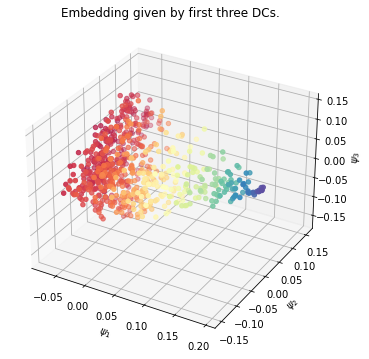
\includegraphics[width=\textwidth]{figures/topology/X1_embedding.png}
    \caption{Three-dimensional embedding of the original point cloud $X_1$.}
\end{subfigure}
\hfill
\begin{subfigure}[b]{0.3\textwidth}
    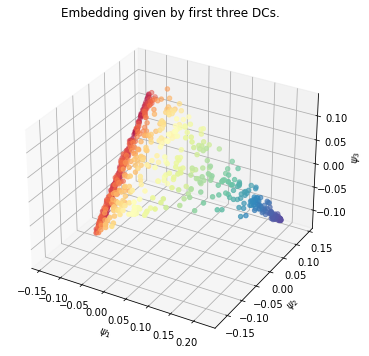
\includegraphics[width=\textwidth]{figures/topology/X2_embedding.png}
    \caption{Three-dimensional embedding of the original point cloud $X_2$.}
\end{subfigure}
\hfill
\begin{subfigure}[b]{0.3\textwidth}
    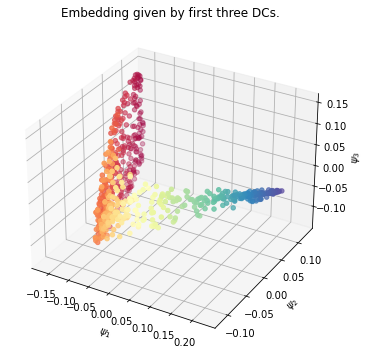
\includegraphics[width=\textwidth]{figures/topology/X3_embedding.png}
    \caption{Three-dimensional embedding of the original point cloud $X_3$.}
\end{subfigure}
\hfill
\begin{subfigure}[b]{0.3\textwidth}
    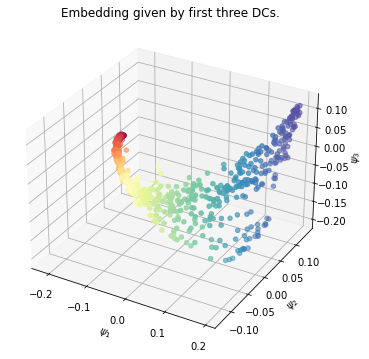
\includegraphics[width=\textwidth]{figures/topology/X4_embedding.png}
    \caption{Three-dimensional embedding of the original point cloud $X_4$.}
\end{subfigure}
\hfill
\begin{subfigure}[b]{0.3\textwidth}
    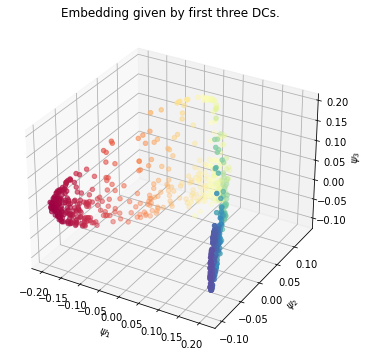
\includegraphics[width=\textwidth]{figures/topology/X5_embedding.png}
    \caption{Three-dimensional embedding of the original point cloud $X_5$.}
\end{subfigure}
\hfill
\begin{subfigure}[b]{0.3\textwidth}
    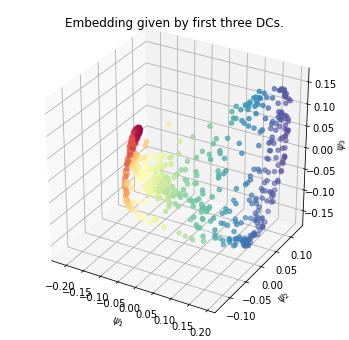
\includegraphics[width=\textwidth]{figures/topology/X6_embedding.png}
    \caption{Three-dimensional embedding of the original point cloud $X_6$.}
\end{subfigure}
\end{figure}

\chapter{Experiments with Artificial Neural Tensors} 
\label{chapter-artifical} 
We generated the neural manifold for artificial neural networks (ANNs) using the same approach as we did for biological neural networks in the previous chapter. But unlike the latter where the neural tensors were already available from the lab experiments, we need to first build the artificial neural tensor by taking the outputs of neuron units in pre-trained ANNs. 

\section{Building the artificial neural tensor}
In the first semester, we have been focusing on investigating the manifold structure of CNN, and specifically the VGG-16 model, but the same method applies to any ANNs. VGG-16 is one of the most successful CNN models in computer vision tasks such as image classification. Its architecture is shown in the figure below. Since previous works have already trained the VGG-16 model to obtain optimal weights, we will directly use the pre-trained weights to generate the artificial neural tensor. 

\begin{figure}[H]
        \centering
            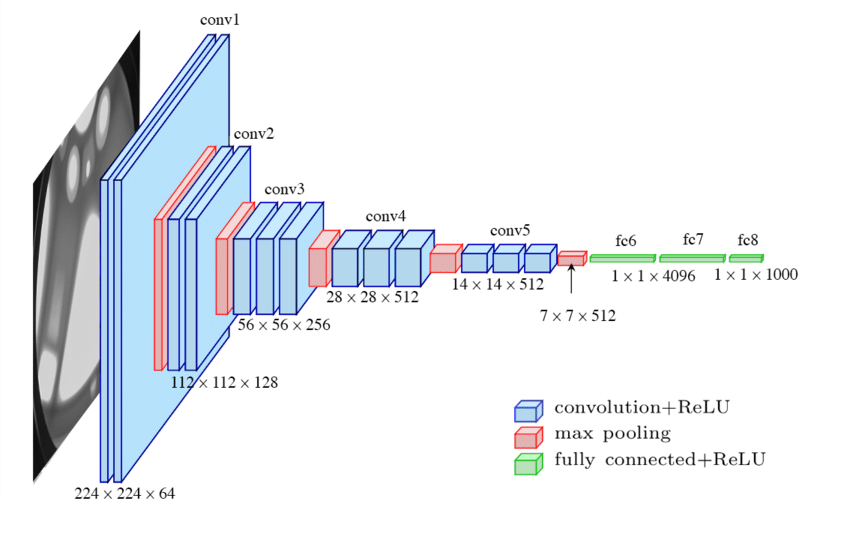
\includegraphics[width=0.9\textwidth]{figures/artificial/vgg16.png}
            \caption{Visualizing the structure of the VGG-16 model.}
    \end{figure}
    
\subsection{``Visual stimuli" in ANNs}
Analogous to the visual flows used in lab experiments, the ``visual stimuli" for ANNs are natural images of different objects (e.g. cars, cats, and dogs) selected from the commonly used data set, CIFAR-10 (\cite{Krizhevsky09cifar-10}). CIFAR-10 consists of 60000 32x32 colour images in 10 classes, with 6000 images per class. To keep the size of the artificial neural tensor manageable, we randomly selected 10 images from each class as the visual stimuli. In order to simulate the movement of visual flows used in lab experiments, we implemented the shifts in image, that is, for every image we shifted the image vertically and horizontally (by one pixel per step). 
    % add image
    \begin{figure}[H]
        \centering
            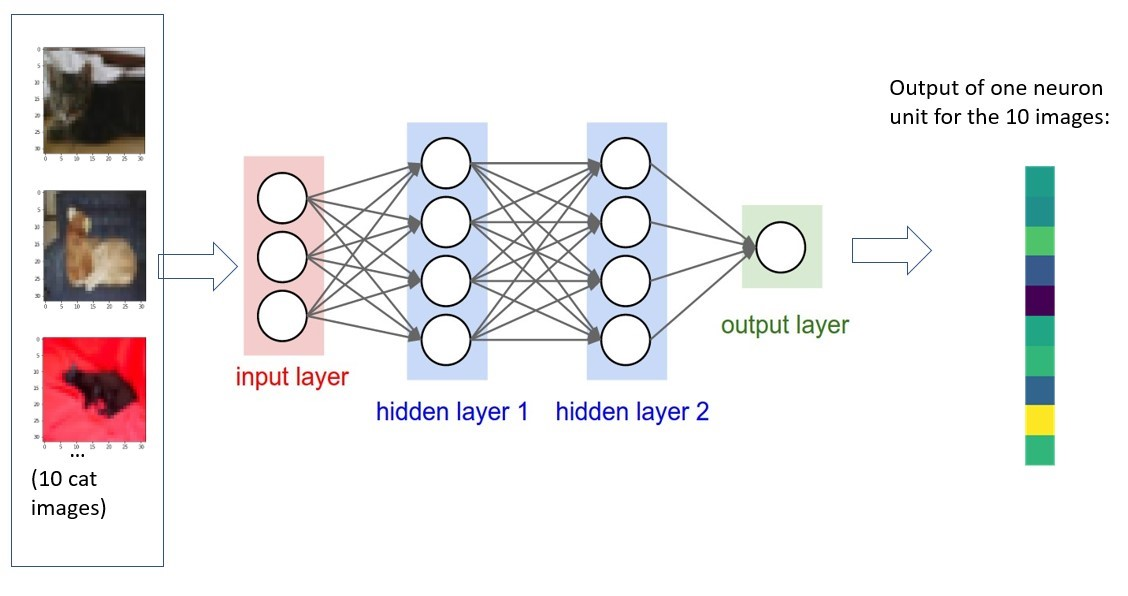
\includegraphics[width=0.9\textwidth]{presentation/Slide1.jpg}
            \caption{Computing output of one neuron unit in the ANNs given 10 input cat images.}
    \end{figure}

\begin{rmk}
At first it might seem that the use of different ``visual stimuli" for biological and artificial neural networks will lead to an unfair comparison. However, this approach is appropriate for the following reason. The mouse visual system was trained on naturalistic visual information and the visual flows used in the lab experiments are also naturalistic. The VGG-16 model was trained on ImageNet, which are very similar to the CIFAR-10 data set that we used for ``visual stimuli" for ANNs. Thus, in both cases, the visual stimuli are similar to what the respective network was trained to recognize.

That being said, we could also adapt the experiments for ANNs to take the same visual flows as the input. In fact, it is on the agenda for the next steps in our project.
\end{rmk}
 
 \subsection{``Individual neuron'' in ANNs}
 In the lab experiments for biological neural networks, moving visual stimuli trigger spikes in the activation potential in the neurons in the retina. The individual neuron response is the firing rate of the neuron which is dependent on the  electrostatics processes that take place in the synapse. The biological neuron is coarsely modeled by the neuron unit in the ANNs. At the ``dendrite," the input is taken from the ``axons" of the connected neurons. The weight of each neuron models the synaptic process in biological neuron. At the ``cell body," all the inputs are multiplied with the weights and summed. We then add the bias term to the sum and apply the non-linear activation function to obtain the final output from this individual neuron unit at the ``axon." The parallel between an individual biological and artificial neuron is shown in the figures below. 
 
 Note that in our experiments, instead of taking the input from previously connected neuron unit, we make a modification by making each neuron unit always take the image vector as the input.
 
  \begin{figure}[H]
        \centering
            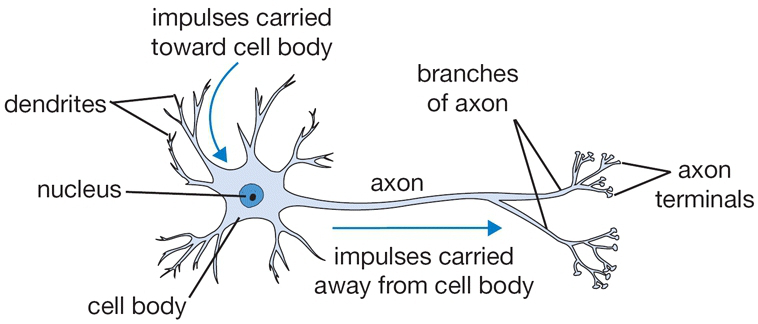
\includegraphics[width=0.9\textwidth]{figures/artificial/neuron.png}
            \caption{An individual neuron in biological neural networks. Adapted from (\cite{cs231n}).}
    \end{figure}
     \begin{figure}[H]
        \centering
            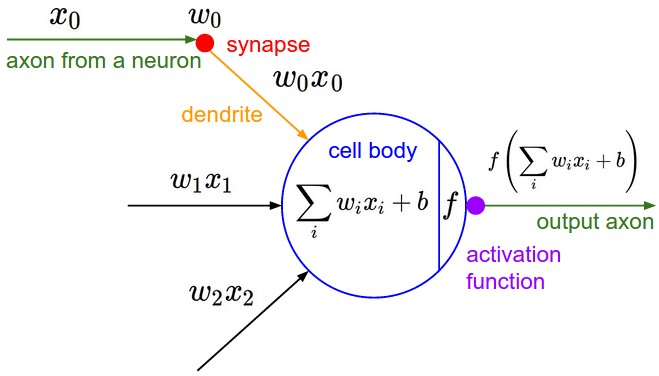
\includegraphics[width=0.9\textwidth]{figures/artificial/neuron_model.jpeg}
            \caption{An ``individual neuron" in ANNs. Adapted from (\cite{cs231n}).}
    \end{figure}
    
\subsection{``Receptive field" of an artificial neuron}
Each layer in the CNN has several different feature maps. Each feature map corresponds to a filter of a specific size and specific weights. The filter is essentially a matrix that, when taking inner product with the input image, give an output that highlights some specific features in the input image. To illustrate this, we can visualize the 64 feature maps in the first convolutional layer of the VGG-16 model, given the input bird image.
\begin{figure}[H]
        \centering
            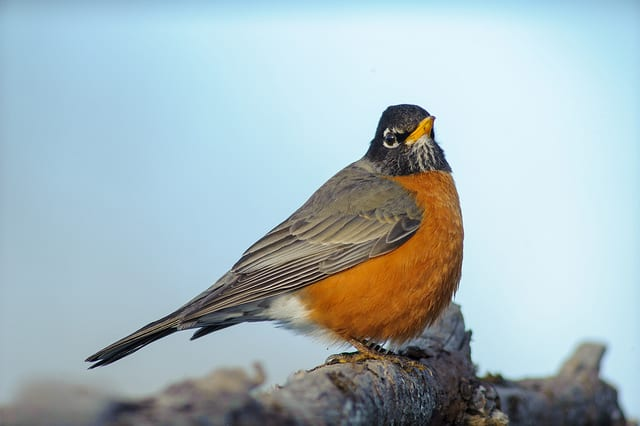
\includegraphics[width=0.9\textwidth]{figures/artificial/bird.jpg}
            \caption{Input image. Adapted from (\cite{feature_map}).}
    \end{figure}
\begin{figure}[H]
        \centering
            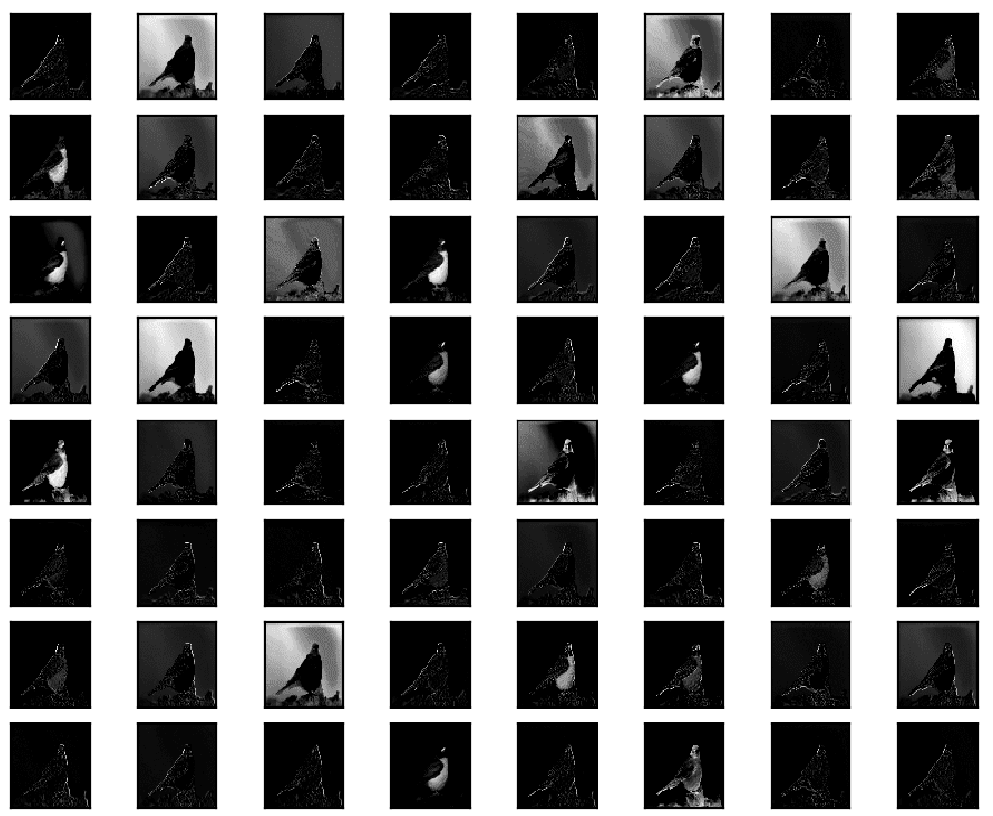
\includegraphics[width=0.9\textwidth]{figures/artificial/feature_map_vgg16.png}
            \caption{Visualizing the 64 feature maps in the first convolutional layer of the VGG-16 model. Adapted from (\cite{feature_map}).}
    \end{figure}
    
Each feature map will have a number of neurons. Each neuron attends to a specific subregion of the image, which is called their ``receptive field." This term in fact originated from the study of the biological visual system, which is defined as a restricted region of visual space where a luminous stimulus could drive electrical responses in a retinal ganglion cell.

The size of the receptive field of is the same as the filter size corresponding to the feature map in which the neuron is located. Each neuron will have the same set of weights as the other neurons in the same feature map (this is sometimes called ``weights sharing"). 

 \subsection{``Neuron population response" in ANNs}
Analogous to the neuron population response in biological neural networks, we computed the all the neuron output given the input image and analyze them collectively, instead of looking at each neuron output individually.

However, one difference from the biological neural networks is that given an image input, most of the neurons will have output of small values (since except for the specific neurons that target at recognizing a specific features, a large number of pre-trained weights are close to zero). In other words, the ``firing" of neurons in ANNs will be sparse. Thus, we selected only ten feature maps with highest average firing rate (the average is taken over all neurons in the respective feature map). 

We now illustrate the dimensions of the resulting artificial neural tensor built from the first convolutional layer of VGG-6. Since there were 1024 neurons in each feature map and we selected 10 feature maps, there were 10240 neurons in total. The visual stimuli consists of 10 images from each of the 10 classes, which give us 100 images. Each of the images have 1024 shifts. In the end, the size of the artificial tensor for the first convolutional layer is thus 10240-by-100-by-1024. 

\section{Applying tensor CP decomposition}
Having built the artificial neural tensor, we then applied the tensor CP decomposition to obtain the first five tensor factors: 
      \begin{figure}[H]
        \centering
            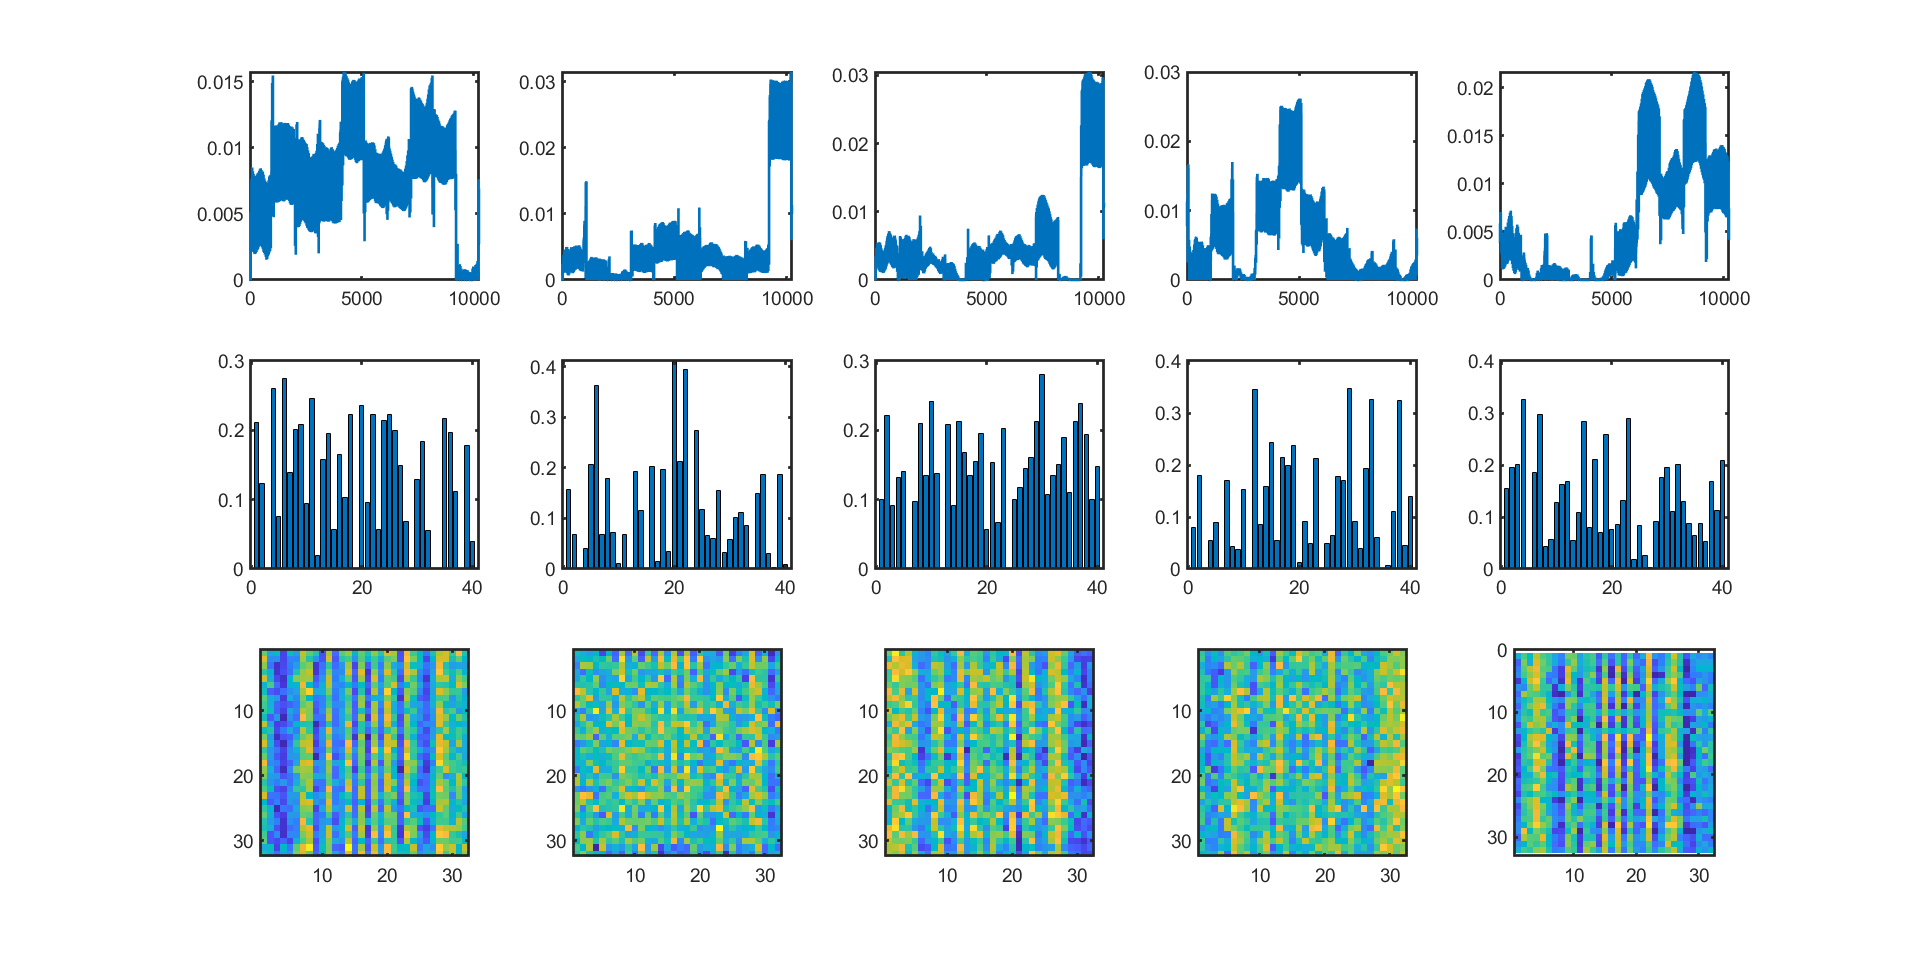
\includegraphics[width=\textwidth]{artificial-tensor/results/nonneg_factors_3D.png}
            \caption{First 5 tensor factors for artificial neural data.}
        \end{figure} 

We then generated the neural manifolds from artificial neural tensor, which can be visualized in the following plot. 
    \begin{figure}[H]
        \centering
            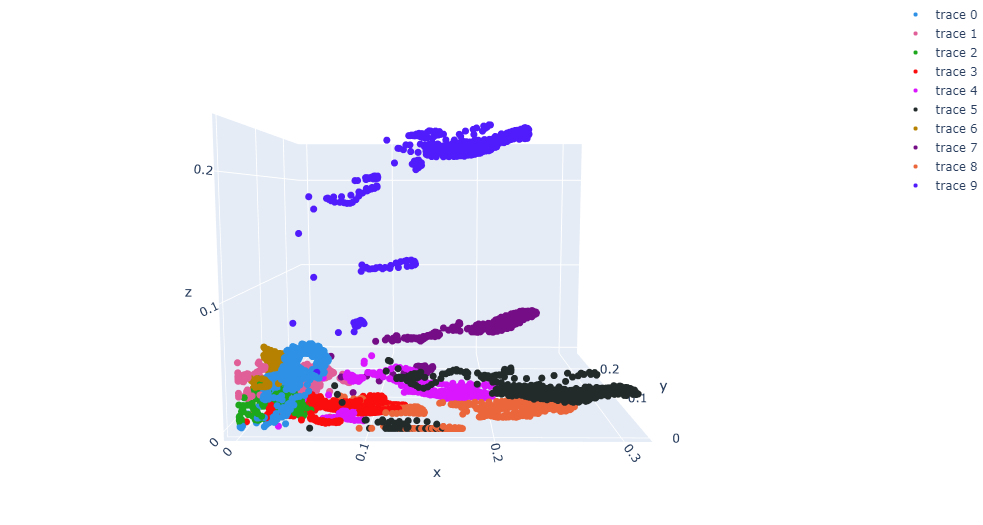
\includegraphics[width=\textwidth]{artificial-tensor/results/TCA_3D.png}
            \caption{Neural manifold generated from artificial neural tensor.}
        \end{figure} 

\chapter{Topological Methods}
\label{chapter-topology} 

\section{Topological data analysis}
This chapter provides the details for an explorative study that extends the method by further extracting topological features from the neural manifolds in response to different visual stimuli. We present here an overview of the steps of our implementation and the results. Full details on the theoretical background of persistent homology can be found in Appendix \ref{AppendixA}. 

Recall that in Chapter 6, we showed the results of using diffusion map to generate the three-dimensional neural manifolds corresponding to six stimuli types, respectively. In this chapter we describe further experiments that investigated the topological structure of the neural manifolds.


\section{Step 1: Applying persistent homology}
We first applied persistent homology to extract the topological features from  the six neural manifolds respectively. In this step, these topological features are represented by persistence barcodes and persistence diagrams.

Our implementation used the package ripser (\cite{ctralie2018ripser}) to obtain the respective persistence diagrams from the embeddings. Using the (birth, death)-intervals from each persistence diagram, we drew the equivalent persistence barcode representation. The complete code can be found in Appendix \ref{AppendixA}. The following figures show the results from applying persistent homology.
\begin{figure}[H]
\centering
\begin{subfigure}[b]{0.2\textwidth}
    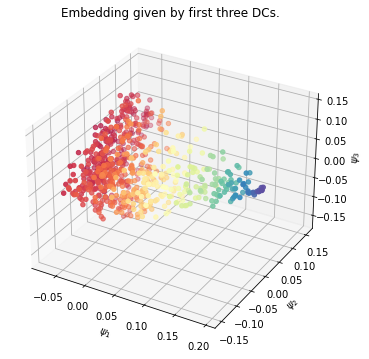
\includegraphics[width=\textwidth]{figures/topology/X1_embedding.png}
    \caption{Three-dimensional embedding of the original point cloud $X_1$.}
\end{subfigure}
\hfill
\begin{subfigure}[b]{0.75\textwidth}
    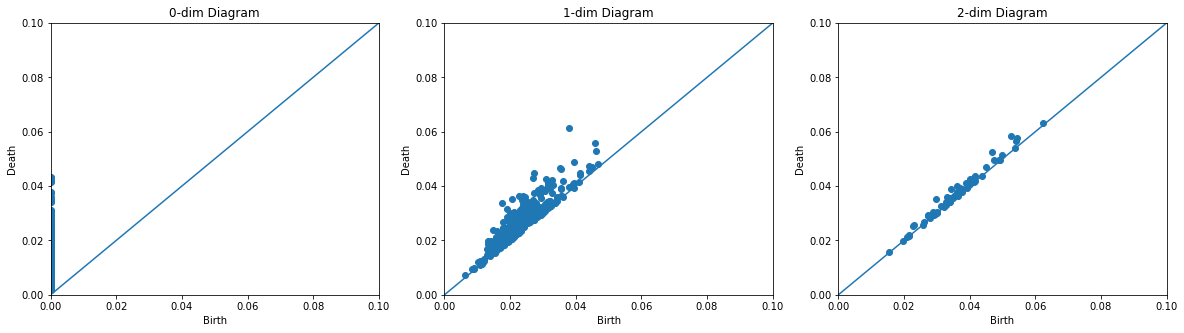
\includegraphics[width=\textwidth]{figures/topology/X1_H0.png}
    \caption{Persistence diagrams.}
\end{subfigure}
\begin{subfigure}[b]{0.25\textwidth}

\includegraphics[width=\textwidth]{figures/topology/white.png} 
\end{subfigure}
\begin{subfigure}[b]{0.24\textwidth}
    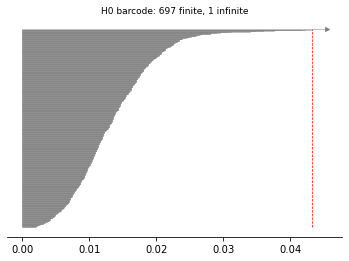
\includegraphics[width=\textwidth]{figures/topology/X1_H0_barcode.png}
    \caption{}
\end{subfigure}
\begin{subfigure}[b]{0.24\textwidth}
    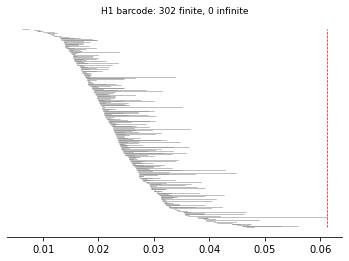
\includegraphics[width=\textwidth]{figures/topology/X1_H1_barcode.png}
        \caption{Persistence barcodes.}
\end{subfigure}
\begin{subfigure}[b]{0.24\textwidth}
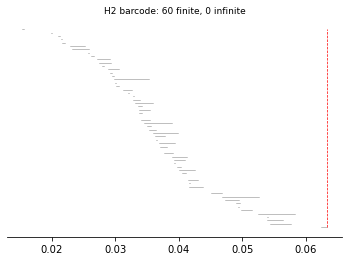
\includegraphics[width=\textwidth]{figures/topology/X1_H2_barcode.png}
 \caption{}
\end{subfigure}
\caption{Results for applying persistent homology on the three-dimensional embedding of $X_1$.}
\end{figure}

\begin{figure}[H]
\centering
\begin{subfigure}[b]{0.2\textwidth}
    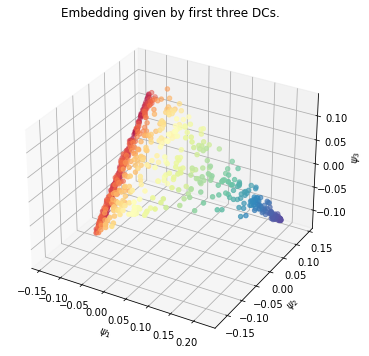
\includegraphics[width=\textwidth]{figures/topology/X2_embedding.png}
    \caption{Three-dimensional embedding of the original point cloud $X_2$.}
\end{subfigure}
\hfill
\begin{subfigure}[b]{0.75\textwidth}
    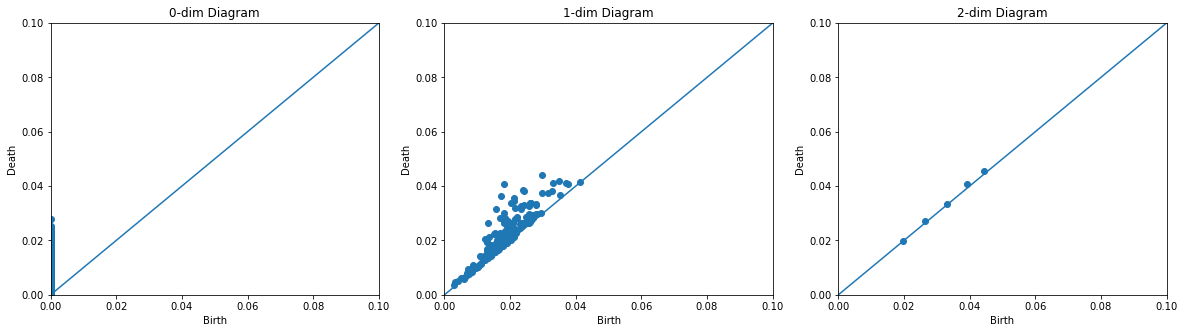
\includegraphics[width=\textwidth]{figures/topology/X2_H0.png}
    \caption{Persistence diagrams.}
\end{subfigure}
\begin{subfigure}[b]{0.25\textwidth}

\includegraphics[width=\textwidth]{figures/topology/white.png} 
\end{subfigure}
\begin{subfigure}[b]{0.24\textwidth}
    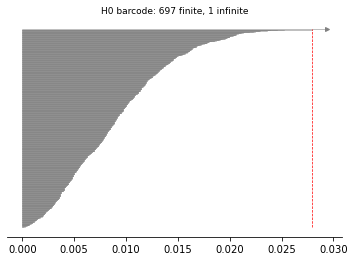
\includegraphics[width=\textwidth]{figures/topology/X2_H0_barcode.png}
    \caption{}
\end{subfigure}
\begin{subfigure}[b]{0.24\textwidth}
    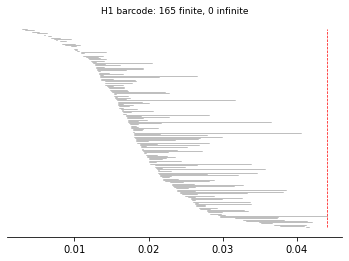
\includegraphics[width=\textwidth]{figures/topology/X2_H1_barcode.png}
        \caption{Persistence barcodes.}
\end{subfigure}
\begin{subfigure}[b]{0.24\textwidth}
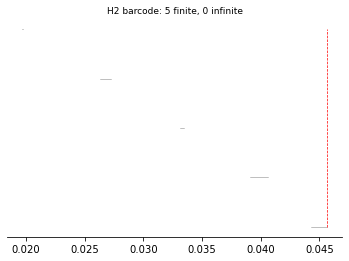
\includegraphics[width=\textwidth]{figures/topology/X2_H2_barcode.png}
 \caption{}
\end{subfigure}
\caption{Results for applying persistent homology on the three-dimensional embedding of $X_2$.}
\end{figure}

\begin{figure}[H]
\centering
\begin{subfigure}[b]{0.2\textwidth}
    \includegraphics[width=\textwidth]{figures/topology/X3_embedding.png}
    \caption{Three-dimensional embedding of the original point cloud $X_3$.}
\end{subfigure}
\hfill
\begin{subfigure}[b]{0.75\textwidth}
    \includegraphics[width=\textwidth]{figures/topology/X3_H0.png}
    \caption{Persistence diagrams.}
\end{subfigure}
\begin{subfigure}[b]{0.25\textwidth}
\includegraphics[width=\textwidth]{figures/topology/white.png} 
\end{subfigure}
\begin{subfigure}[b]{0.24\textwidth}
    \includegraphics[width=\textwidth]{figures/topology/X3_H0_barcode.png}
    \caption{}
\end{subfigure}
\begin{subfigure}[b]{0.24\textwidth}
    \includegraphics[width=\textwidth]{figures/topology/X3_H1_barcode.png}
        \caption{Persistence barcodes.}
\end{subfigure}
\begin{subfigure}[b]{0.24\textwidth}
\includegraphics[width=\textwidth]{figures/topology/X3_H2_barcode.png}
 \caption{}
\end{subfigure}
\caption{Results for applying persistent homology on the three-dimensional embedding of $X_3$.}
\end{figure}

\begin{figure}[H]
\centering
\begin{subfigure}[b]{0.2\textwidth}
    \includegraphics[width=\textwidth]{figures/topology/X4_embedding.png}
    \caption{Three-dimensional embedding of the original point cloud $X_4$.}
\end{subfigure}
\hfill
\begin{subfigure}[b]{0.75\textwidth}
    \includegraphics[width=\textwidth]{figures/topology/X4_H0.png}
    \caption{Persistence diagrams.}
\end{subfigure}
\begin{subfigure}[b]{0.25\textwidth}
\includegraphics[width=\textwidth]{figures/topology/white.png} 
\end{subfigure}
\begin{subfigure}[b]{0.24\textwidth}
    \includegraphics[width=\textwidth]{figures/topology/X4_H0_barcode.png}
    \caption{}
\end{subfigure}
\begin{subfigure}[b]{0.24\textwidth}
    \includegraphics[width=\textwidth]{figures/topology/X4_H1_barcode.png}
        \caption{Persistence barcodes.}
\end{subfigure}
\begin{subfigure}[b]{0.24\textwidth}
\includegraphics[width=\textwidth]{figures/topology/X4_H2_barcode.png}
 \caption{}
\end{subfigure}
\caption{Results for applying persistent homology on the three-dimensional embedding of $X_4$.}
\end{figure}

\begin{figure}[H]
\centering
\begin{subfigure}[b]{0.2\textwidth}
    \includegraphics[width=\textwidth]{figures/topology/X5_embedding.png}
    \caption{Three-dimensional embedding of the original point cloud $X_5$.}
\end{subfigure}
\hfill
\begin{subfigure}[b]{0.75\textwidth}
    \includegraphics[width=\textwidth]{figures/topology/X5_H0.png}
    \caption{Persistence diagrams.}
\end{subfigure}
\begin{subfigure}[b]{0.25\textwidth}
\includegraphics[width=\textwidth]{figures/topology/white.png} 
\end{subfigure}
\begin{subfigure}[b]{0.24\textwidth}
    \includegraphics[width=\textwidth]{figures/topology/X5_H0_barcode.png}
    \caption{}
\end{subfigure}
\begin{subfigure}[b]{0.24\textwidth}
    \includegraphics[width=\textwidth]{figures/topology/X5_H1_barcode.png}
        \caption{Persistence barcodes.}
\end{subfigure}
\begin{subfigure}[b]{0.24\textwidth}
\includegraphics[width=\textwidth]{figures/topology/X5_H2_barcode.png}
 \caption{}
\end{subfigure}
\caption{Results for applying persistent homology on the three-dimensional embedding of $X_5$.}
\end{figure}

\begin{figure}[H]
\centering
\begin{subfigure}[b]{0.2\textwidth}
    \includegraphics[width=\textwidth]{figures/topology/X6_embedding.png}
    \caption{Three-dimensional embedding of the original point cloud $X_6$.}
\end{subfigure}
\hfill
\begin{subfigure}[b]{0.75\textwidth}
    \includegraphics[width=\textwidth]{figures/topology/X6_H0.png}
    \caption{Persistence diagrams.}
\end{subfigure}
\begin{subfigure}[b]{0.25\textwidth}
\includegraphics[width=\textwidth]{figures/topology/white.png} 
\end{subfigure}
\begin{subfigure}[b]{0.24\textwidth}
    \includegraphics[width=\textwidth]{figures/topology/X6_H0_barcode.png}
    \caption{}
\end{subfigure}
\begin{subfigure}[b]{0.24\textwidth}
    \includegraphics[width=\textwidth]{figures/topology/X6_H1_barcode.png}
        \caption{Persistence barcodes.}
\end{subfigure}
\begin{subfigure}[b]{0.24\textwidth}
\includegraphics[width=\textwidth]{figures/topology/X6_H2_barcode.png}
 \caption{}
\end{subfigure}
\caption{Results for applying persistent homology on the three-dimensional embedding of $X_6$.}
\end{figure}

\section{Step 2: Pairwise Wasserstein distance}
In this step, we used the gudhi package (\cite{gudhi:urm}) to compute the pairwise Wasserstein distance between the persistence diagrams. The method used is based on (\cite{kerber_geometry_2016}). 

We first computed the first pairwise distances between the persistence diagrams for each of the six point clouds. 

\begin{table}[!htbp]
        \centering
        \small
        \setlength\tabcolsep{5pt}
        \begin{tabular}{|c|c|c|c|c|c|c|}
\hline
 $H_0$& $X_1$ & $X_2$ & $X_3$ & $X_4$ & $X_5$ & $X_6$\\
 \hline
$X_1$ &
0.0&
2.77&
3.05&
3.95&
3.08&
3.42
\\
\hline
$X_2$ &
2.77&
0.0&
0.43&
1.35&
1.0&
0.84
\\
\hline
$X_3$ &
3.05&
0.43&
0.0&
1.03&
0.94&
0.66
\\
\hline
$X_4$ &
3.95&
1.35&
1.03&
0.0&
1.11&
0.72
\\
\hline
$X_5$ &
3.08&
1.0&
0.94&
1.11&
0.0&
0.51
\\
\hline
$X_6$ &
3.42&
0.84&
0.66&
0.72&
0.51&
0.0
\\
\hline
\end{tabular}
\caption{Pairwise Wasserstein distance between persistent diagrams for homology group $H_0$.}
\label{tab:Wass_H0}
\end{table}

\begin{table}[!htbp]
        \centering
        \small
        \setlength\tabcolsep{5pt}
        \begin{tabular}{|c|c|c|c|c|c|c|}
\hline
 $H_1$& $X_1$ & $X_2$ & $X_3$ & $X_4$ & $X_5$ & $X_6$ \\ \hline
$X_1$ &
0.0&
0.46&
0.5&
0.64&
0.64&
0.55

\\\hline
$X_2$ &
0.46&
0.0&
0.17&
0.29&
0.36&
0.3
\\\hline
$X_3$ &
0.5&
0.17&
0.0&
0.25&
0.33&
0.3
\\\hline 
$X_4$ &
0.64&
0.29&
0.25&
0.0&
0.27&
0.29
\\\hline 
$X_5$ &
0.64&
0.36&
0.33&
0.27&
0.0&
0.26

\\\hline
$X_6$ &
0.55&
0.3&
0.3&
0.29&
0.26&
0.0\\
\hline
\end{tabular}
\caption{Pairwise Wasserstein distance between persistent diagrams for homology group $H_1$.}
\label{tab:Wass_H1}
\end{table}

\begin{table}[!htbp]
        \centering
        \small
        \setlength\tabcolsep{5pt}
        \begin{tabular}{|c|c|c|c|c|c|c|}
\hline
 $H_2$& $X_1$ & $X_2$ & $X_3$ & $X_4$ & $X_5$ & $X_6$ \\ \hline
$X_1$ &
0.0&
0.06&
0.06&
0.06&
0.06&
0.06
\\
\hline
$X_2$ &
0.06&
0.0&
0.01&
0.0&
0.01&
0.0
\\
\hline
$X_3$ &
0.06&
0.01&
0.0&
0.0&
0.01&
0.0
\\
\hline
$X_4$ &
0.06&
0.0&
0.0&
0.0&
0.0&
0.0
\\
\hline
$X_5$ &
0.06&
0.01&
0.01&
0.0&
0.0&
0.0
\\
\hline
$X_6$ &
0.06&
0.0&
0.0&
0.0&
0.0&
0.0
\\
\hline
\end{tabular}
\caption{Pairwise Wasserstein distance between persistent diagrams for homology group $H_2$.}
\label{tab:Wass_H2}
\end{table}

Building upon the same method, we further compared the six point clouds with known three-dimensional shapes ($2$-sphere and torus) based on the Wasserstein distance.

First, we extracted the topological features of the $2$-sphere and three-dimensional torus, as we did for the point clouds in Step 2. 
\begin{figure}[H]
\centering
\begin{subfigure}[b]{0.2\textwidth}
    \includegraphics[width=\textwidth]{figures/topology/dsphere.png}
    \caption{Scatter plot for $2$-sphere.}
\end{subfigure}
\hfill
\begin{subfigure}[b]{0.75\textwidth}
    \includegraphics[width=\textwidth]{figures/topology/dsphere_Hk.png}
    \caption{Persistence diagrams.}
\end{subfigure}
\begin{subfigure}[b]{0.25\textwidth}
\includegraphics[width=\textwidth]{figures/topology/white.png} 
\end{subfigure}
\begin{subfigure}[b]{0.24\textwidth}
    \includegraphics[width=\textwidth]{figures/topology/dsphere_H0_barcode.png}
    \caption{}
\end{subfigure}
\begin{subfigure}[b]{0.24\textwidth}
    \includegraphics[width=\textwidth]{figures/topology/dsphere_H1_barcode.png}
        \caption{Persistence barcodes.}
\end{subfigure}
\begin{subfigure}[b]{0.24\textwidth}
\includegraphics[width=\textwidth]{figures/topology/dsphere_H2_barcode.png}
 \caption{}
\end{subfigure}
\caption{Results for applying persistent homology on the $2$-sphere.}
\end{figure}

\begin{figure}[H]
\centering
\begin{subfigure}[b]{0.2\textwidth}
    \includegraphics[width=\textwidth]{figures/topology/torus.png}
    \caption{Scatter plot for the three-dimensional torus.}
\end{subfigure}
\hfill
\begin{subfigure}[b]{0.75\textwidth}
    \includegraphics[width=\textwidth]{figures/topology/torus_Hk.png}
    \caption{Persistence diagrams.}
\end{subfigure}
\begin{subfigure}[b]{0.25\textwidth}
\includegraphics[width=\textwidth]{figures/topology/white.png} 
\end{subfigure}
\begin{subfigure}[b]{0.24\textwidth}
    \includegraphics[width=\textwidth]{figures/topology/torus_H0_barcode.png}
    \caption{}
\end{subfigure}
\begin{subfigure}[b]{0.24\textwidth}
    \includegraphics[width=\textwidth]{figures/topology/torus_H1_barcode.png}
        \caption{Persistence barcodes.}
\end{subfigure}
\begin{subfigure}[b]{0.24\textwidth}
\includegraphics[width=\textwidth]{figures/topology/torus_H2_barcode.png}
 \caption{}
\end{subfigure}
\caption{Results for applying persistent homology on the three-dimensional torus.}
\end{figure}

Then, we computed the Wasserstein distance between the six point clouds and the known shapes:

\begin{table}[!htbp]
        \centering
        \small
        \setlength\tabcolsep{5pt}
        \begin{tabular}{|c|c|c|c|c|c|c|}
\hline
  $H_0$& $X_1$ & $X_2$ & $X_3$ & $X_4$ & $X_5$ & $X_6$ \\ \hline
$2$-sphere & 2.48 & 4.46&  4.64 & 5.18 & 4.53 & 4.83\\\hline
torus & 3.63 &  1.46 & 1.31 & 0.73 & 1.38 & 1.06 \\ \hline
\end{tabular}
\caption{Wasserstein distance between persistent diagrams of the point clouds and $2$-sphere and torus (homology group $H_0$).}
\label{tab:sphere-H0}
\end{table}


\begin{table}[!htbp]
        \centering
        \small
        \setlength\tabcolsep{5pt}
        \begin{tabular}{|c|c|c|c|c|c|c|}
\hline
$H_1$& $X_1$ & $X_2$ & $X_3$ & $X_4$ & $X_5$ & $X_6$ \\ \hline
$2$-sphere & 0.62 &   0.77 & 0.80 & 0.87 & 0.85 & 0.76\\\hline
torus & 0.74 & 0.49 & 0.44 & 0.34 & 0.45 & 0.47\\ \hline
\end{tabular}
\caption{Wasserstein distance between persistent diagrams of the point clouds and $2$-sphere and torus (homology group $H_1$).}
\label{tab:sphere-H1}
\end{table}

\begin{table}[!htbp]
        \centering
        \small
        \setlength\tabcolsep{5pt}
        \begin{tabular}{|c|c|c|c|c|c|c|}
\hline
$H_2$ & $X_1$ & $X_2$ & $X_3$ & $X_4$ & $X_5$ & $X_6$ \\ \hline
$2$-sphere & 0.11 &   0.12 & 0.12 & 0.12 & 0.13 & 0.12\\\hline
torus & 0.057 & 0.017 & 0.018  & 0.016 & 0.018 & 0.016 \\ \hline
\end{tabular}
\caption{Wasserstein distance between persistent diagrams of the point clouds and $2$-sphere and torus (homology group $H_2$).}
\label{tab:sphere-H2}
\end{table}

\section{Analysis of results}
Based on the results from the above tables of Wasserstein distances, our observations and inferences are as follows.

\begin{enumerate}
    \item The topological structure for $X_1$ is distinct from the rest. 
    
    Based on the pairwise Wasserstein distances in Tables \ref{tab:Wass_H0} and \ref{tab:Wass_H1}, $X_1$ is notably different from the rest of the point clouds in terms of topological structure. In the context of our application, this implies that the neural population response evoked by stimulus type 1 is significantly different from the other stimulus types. This observation leads us to hypothesize that there is some neuroscientific reason behind this distinction in the topological structure of neural population response. It might be interesting to conduct further lab experiments to investigate what special properties this stimulus has and why it causes such different  neural population response. 
    
    \item Wasserstein distances between persistence diagrams are nearly negligible for $H_2$.
    
    Based on Table \ref{tab:Wass_H2}, pairwise Wasserstein distances between persistence diagrams for $H_2$ are small enough to be nearly negligible. This implies that the intrinsic dimensionality of this neural data might be even lower than three-dimensional since there is no significant differences in homology groups $H_2$ for the point clouds.
    
    \item Shape comparison with $2$-sphere and torus.
    
    Based on Tables \ref{tab:sphere-H0} and \ref{tab:sphere-H1}, the Wasserstein distances between the point clouds and the $2$-sphere are smaller than the Wasserstein distances between the point clouds and the torus for all $X_i$ except for $X_1$. We can thus infer that except for $X_1$, all other point clouds are more similar to the shape of a torus than the $2$-sphere. This implies that the topological structure of the neural population response evoked by stimuli type 1 is more similar to a sphere while the neural population response evoked by the rest of the stimuli types used in the experiments are more similar to a torus. 
    
    It would be interesting to compare this result with the hypothesis in (\cite{ben-yishai_theory_1995}, \cite{Blumenfeld_2006}, \cite{goldberg_randomized_2004},    \cite{singh_top_v1_2008}):
    If we are given an oriented stimulus, and if the orientation is a circular variable, then the hypothesis is that the neural population response evoked by such stimulus must have a topological structure equivalent to that of a circle. However, to fully test this hypothesis, further experiments with different types of stimuli need to be conducted.
\end{enumerate}

\section{Discussions}
In this chapter, we demonstrated our proposed approach to compare the point clouds that represent the neural population response to different stimuli. Our proposed approach is contingent on the topological structures of the point clouds.  

One significant limitation in this specific application is that lab data usually involve a lot of sampling errors such as missing data and inconsistent densities, causing noise to the true underlying geometry of the neural population response. Persistent homology works well on synthetic data, but might not work when the sampling errors are too significant.

The advantages of topological approach is that we can provide a succinct and useful summary of the global geometric structure of the neural spiking data, thus obtaining a useful account of how similarly the neurons collectively respond to visual stimuli. This is especially important in applications where the notion of connectedness and clusters are salient. As an emerging field, TDA will certainly see more applications in solving problems that involve understanding the geometric and topological structure of high-dimensional data.

\chapter{Conclusion}
\label{chapter-conclusion} 

\section{Summary of work done}

In the first semester, the main objective is to develop proficiency in the necessary theoretical foundation and implementation skills. These included tensor CP decomposition, diffusion map, and persistent homology. To gain better intuition, I demonstrated each of the methods on toy data sets such as face image data and MNIST \cite{mnist}. 

Due to the interdisciplinary nature of the project, much time is also spent studying the theoretical foundations of computational neuroscience. This includes the history of computational models of the visual system and the connections with mathematical and computational ideas. 

I have also conducted many exploratory experiments. A complete list of the experiments are included below.
For the biological neural tensor, I conducted the following experiments:
\begin{enumerate}
    \item applying tensor CP decomposition to generate the neural manifold
    \item applying diffusion map to generate the neural manifold
    \item applying persistent homology and Wasserstein distance to compare the topological features of the neural manifold
\end{enumerate}

For the artificial neural tensor, I conducted the following experiments:
\begin{enumerate}
    \item building the artificial neural tensor without considering shifts in images
    \item building the artificial neural tensor with shifts in images
    \item applying tensor CP decomposition on the artificial neural tensor (with shifts in images)
    \item studying how the neural manifold changes during the training of an ANN (instead of using the pre-trained ANN)
    \item applying persistent homology (though with limited explainability)
\end{enumerate}

In all, I am on track with the timeline and have completed more than the plans we laid out at the beginning of the semester.  A bird-eye view of the work done during the first semester is shown in the figure below.

\begin{figure}[H]
        \centering
     \includegraphics[width=1.2\textwidth]{presentation/Slide4.jpg}
        \end{figure} 
        
\section{Next steps}
In the past few months, I have finished learning the foundations behind the methods and applying these methods to conduct relevant experiments using the neural tensors from the lab neural spiking data and the pre-trained VGG-16 model.  

Given the progress made, I propose the following next steps:
\begin{itemize}
    \item Provide more thorough and rigorous interpretations of the results for CNN. This will likely involve more sophisticated understanding of theoretical neuroscience, which could be addressed by reading the book on neuromathemtics and talking to the co-supervisor who is working directly in this area. 
    \item Apply the same methods to RNN to investigate whether there would be any interesting differences.
    \item Come up with a way to quantify the differences between neural manifolds. This could potentially be done by using persistent homology and the Wasserstein distance.
    \item Implement diffusion map on the artificial neural tensors with the appropriate parameters.
    \item Identify a potential novelty that this project could offer, which would be a contribution that is not in the research literature before. This could be some interesting results from the experiments, or a proposal of a new improvement to the existing methodology. 
\end{itemize}





\printbibliography[heading=bibintoc]

\appendix 
 \chapter{Persistent Homology Theory} 
\label{AppendixA} 

In this appendix, we provide the full details on the theoretical background of persistent homology.
The main references for the following exposition are (\cite{carlsson_topology_2009}) and (\cite{zomorodian_computing_nodate}).

\section{Motivation}

First of all, there are four major advantages for using topological methods to analyze high-dimensional point clouds.

\begin{enumerate}
	\item Topology provides qualitative information which is required for data analysis.
	
	\item Metrics are not theoretically justified. Compared to straightforward geometric methods, Topology is less sensitive to the actual choice of metrics. 
	
	\item Studying geometric objects using Topology does not depend on the coordinates. 
	
	\item Functoriality. This is the most important advantage.
	
	\begin{defn}[Functoriality]
	
		For any topological space X, abelian group $A$, and integer $k\geq 0,$ there is assigned a group $H_k(X,A).$ For any $A$ and $k$, and any continuous map $f: X \to Y,$ there is an induced homomorphism $H_k(f,A): H_k(X,A) \to H_k(Y,A).$ Then \underline{functoriality} refers to the following conditions:
		\begin{itemize}
			\item  $H_k(f\circ g,A): H_k(f,A) \circ H_k(g,A)$
			\item  $H_k(Id_{X};A) = Id_{H_k(X,A)}.$
		\end{itemize}
	\end{defn}
	Functoriality addresses the ambiguities in statistical clustering methods -- in particular the arbitrariness of various threshold choices. We now illustrate how exactly functoriality could be used in questions related to clustering. 
	
	Let $X$ be the full data set and $X_1,X_2$ are the subsamples from the data set. If the set of clusterings $C(X_1), C(X_2), C(X_1 \cup X_2)$ correspond well, then we can conclude that the subsample clusterings correspond to clusterings in the full data set $X$. 
\end{enumerate}

\section{Homotopy} \label{sec:homotopy}

\begin{defn}[Homotopy]

	\underline{Homotopy} is a family of maps $f_t: X \to Y$ where $t \in I$ such that $F: X\times I \to Y$ defined by $F(x,t) \mapsto f_t(x)$ is continuous.
	
	Two maps $f_0, f_1$ are \underline{homotopic} if there exists a homotopy $f_t$ between $f_0$ and $f_1$.  
\end{defn}

\begin{defn}[Homotopy equivalence]
A map $f:X \to Y$ is a \underline{homotopy equivalence} if there is a map $g: Y \to X$ such that 
\begin{itemize}
	\item $f\circ g$ is homotopic to the identity map on $Y$, and
	\item $g\circ f$ is homotopic to $f$.
\end{itemize}

Two spaces $X,Y$ are\textit{ homotopy equivalent} if there exists a homotopy equivalence $f: X \to Y. $
\end{defn}

\begin{thm}
	If $f$ and $g$ are homotopic, then $H_k(f,A) = H_k(g,A).$ 
	
	If $X$ and $Y$ are homotopy equivalent, then $H_k(X,A) \cong H_k(Y,A) $.
	
	Note that if two spaces are homotopy equivalent, then all their Betti numbers (defined in subsequent section) are equal.
\end{thm}
\begin{defn}[Topological space]
    Associated to a simplicial complex $(V, \triangle)$ is a topological space $|(V,\triangle)|$. $|(V,\triangle)|$ may be defined using a bijection $\phi : V \to \{1, 2, \dots,N\}$ as the subspace of $\mathbb{R}^N$ given by the union 
	$$\bigcup_{\sigma \in \triangle} c(\sigma),$$
	where $c(\sigma)$ is the convex hull of the set $\{e_{\phi(s)}\}_{s\in \sigma}$, where $e_i$ denotes the $i$-th standard basis vector.

	 We often use abstract simplicial complexes to approximate topological spaces. For simplicial complexes the homology can be computed using only the linear algebra of finitely generated $\mathbb{Z}$-modules. In particular, for simplicial complexes, homology is algorithmically computable.
\end{defn}	
	
\begin{defn}[Nerve]
	Let $X$ be a topological space, and let $\mathcal{U} = \{U_\alpha\}_{\alpha\in A}$ be any covering of $X$. 
	
	The \underline{nerve} of $\mathcal{U}$, denoted by $N(\mathcal{U})$, will be the abstract simplicial complex with vertex set $A$, and where a family $\{\alpha_0, \dots, \alpha_k\}$ spans a $k$-simplex if and only if $U_{\alpha_0}\cap U_{\alpha_1} \cap \cdots \cap U_{\alpha_k} \neq \emptyset.$
\end{defn}

One reason that this construction is very useful in the following ``Nerve Theorem." This theorem gives the criteria for $N(\mathcal{U})$ to be homotopy equivalent to the underlying topological space $X$.

\begin{thm}[Nerve Theorem]
Suppose that $X$ and $U$ are as above, and suppose that the covering consists of open sets and is numerable. Suppose further that for all $\emptyset \subseteq A,$ we have that $\bigcap_{s\in S} U_s$ is either contractible or empty. Then $N(\mathcal{U})$ is homotopy equivalent to $X$.
\end{thm}
The Nerve Theorem is very important in TDA since it provides a way to encode the topology of continuous spaces into abstract combinatorial structures that are more useful for designing computationally efficient data structures and algorithms.

\section{Simplicial Complexes}

\begin{defn}[Simplicial complex]

	An \underline{abstract simplicial complex} is a pair $(V, \triangle)$, where $V$ is a finite set, and $\triangle$ is a family of non-empty subsets of $V$ such that 
	$$\tau \in \triangle \text{ and }\sigma \subseteq \tau \implies \sigma \in \triangle.$$
	
	$\tau \in \triangle $ is face of $\triangle$. The dimension of a face $\tau$ is $|\tau| - 1.$
	
	(Intuition) A simplicial complex $\triangle$ in $\mathbb{R}^n$ is a collection of simplices in $\mathbb{R}^n$ such that
	\begin{enumerate}
	    \item Every face of a simplex of $\triangle$ is in $\triangle$.
	    \item The intersection of any two simplicies of $\triangle$ is a face of each. 
	\end{enumerate}
\end{defn}

\begin{defn}[f-vector]

    For each $n \geq -1,$ let $f_n = f_n(\triangle)$ be the number of faces of $\triangle$ of dimension $n$.
    
    The f-vector of $\triangle$ is the vector $(f_{-1}, f_0, f_1, \dots, f_d)$ where $d$ is the dimension of $\triangle$. 
    
    \begin{eg}
    Suppose the family of sets 
    $$\emptyset, \{a\},\{b\},\{c\}, \{d\}, \{a,b\}, \{a,c\}, \{b,c\}, \{b,d\}, \{c,d\}, \{a,b,c\}$$ form a simplicial complex $E_1$. Then the f-vector of $E_1$ is $(1,4,5,1)$.
    \end{eg}
\end{defn}

\begin{defn}[Oriented complex]

(Intuition) An \underline{oriented simplex} is a simplex $\sigma$ together with an orientation of $\sigma$. If $\{a_0, a_1, \dots, a_p\}$ spans a $p$-complex $\sigma$, then we denote the oriented simplex with $[a_0, a_1, \dots, a_p]$.

(Formal) Let $\mathbb{F}$ be a commutative ring, $\triangle$ be a simplicial complex. For each $n \geq -1,$ we form a free $\mathbb{F}$-module $\Chain_n(\triangle; \mathbb{F})$ with a basis indexed by the $n$-dimensional faces of $\triangle$. For each n-dimensional face $a_0 a_1\cdots a_n$, we have a basis element $\vec{e}_{a_0,a_1,\cdots, a_n}$. 

We refer to the basis element $\vec{e}_{a_0,a_1,\cdots, a_n}$ as an \underline{oriented simplex}. The concept of an oriented simplex is analogous to the idea of a unit vector (which gives the direction and has unit length).
\end{defn}

\begin{defn}[Chain group of degree $n$]
    We refer to the free $\mathbb{F}$-module $\Chain_n(\triangle; \mathbb{F})$ in the previous definition as the chain group of degree $n$. The rank of  $\Chain_n(\triangle; \mathbb{F})$ is the $n$-th value $f_n(\triangle)$ in the f-vector of $\triangle$.

\begin{eg}
For $E_1 = \{\emptyset, \{a\},\{b\},\{c\}, \{d\}, \{a,b\}, \{a,c\}, \{b,c\}, \{b,d\}, \{c,d\}, \{a,b,c\}\}$, we have the following chain groups of degrees $-1,0,1,2$, respectively:
\begin{itemize}
    \item $\Chain_{-1}(E_1) = \{\lambda e_{\emptyset}: \lambda \in \mathbb{F}\} \cong \mathbb{F}.$
    \item $\Chain_{0}(E_1) = \{\lambda_{a} e_{a} + \lambda_{b} e_{b}  + \lambda_{c} e_{c} + \lambda_{d} e_{d}: \lambda_{a}, \lambda_{b}, \lambda_{c}, \lambda_{d} \in \mathbb{F}\} \cong \mathbb{F}^4.$
    \item $\Chain_{1}(E_1) = \{\lambda_{a b} e_{a,b} + \cdots  + \lambda_{c d} e_{c,d} : \lambda_{a b}, \dots,  \lambda_{c d} \in \mathbb{F}\} \cong \mathbb{F}^5.$
    \item $\Chain_{2}(E_1) = \{\lambda e_{a,b,c}: \lambda \in \mathbb{F}\} \cong \mathbb{F}.$
\end{itemize}
\end{eg}
\end{defn}

\begin{defn}[Simplicial chain complex]
The \underline{simplicial chain complex} of a simplicial comlex $\triangle$, denoted with $C(\triangle)$, is defined as:

\begin{tikzcd}[cells={nodes={minimum height=2em}}]
\cdots\arrow[r,"\partial_{n+2}"] & 
\Chain_{n+1}(\triangle) \arrow[r,"\partial_{n+1}"] & 
\Chain_{n}(\triangle) \arrow[r,"\partial_{n}"] & 
\Chain_{n-1}(\triangle) \arrow[r,"\partial_{n - 1}"] &
\cdots
\end{tikzcd}

\begin{eg}
The simplicial chain complex of $E_1$,  $C(E_1)$ is 

\begin{tikzcd}[cells={nodes={minimum height=2em}}]
0\arrow[r] & 
\Chain_{2}(E_1) \arrow[r,"\partial_{2}"] \arrow[d, "\cong"] & 
\Chain_{1}(E_1) \arrow[r,"\partial_{1}"] \arrow[d, "\cong"] & 
\Chain_{0}(E_1) \arrow[r,"\partial_{0}"] \arrow[d, "\cong"] &
\Chain_{-1}(E_1) \arrow[r] \arrow[d, "\cong"] &
0\\
0\arrow[r] & \mathbb{F} \arrow[r,"\partial_{2}"] & \mathbb{F}^5  \arrow[r,"\partial_{1}"] & \mathbb{F}^4 \arrow[r,"\partial_{0}"] &
\mathbb{F}  \arrow[r] &
0
\end{tikzcd}
Recall that $E_1$ has f-vector $(1,4,5,1)$.
\end{eg}
\end{defn}
\begin{prop}[The double boundary condition]
\label{double-boundary}
Boundary maps satisfy the double boundary condition, that is, $\partial_n \circ \partial_{n+1} = 0 \quad \forall n.$
\end{prop}
\begin{defn}[Simplicial homology of degree $k$]
\label{kth-homology-group}
    (Intuition) The simplicial homology gives an algebraic measure on the amount of cycles that are not the boundaries. 

    (Formal) Define he $\mathbb{F}$-module $Z_k(\triangle; \mathbb{F})$ of cycles and the $\FF$-module of he boundary group $B_k(\triangle;\FF)$ by the following formulas:
    \begin{itemize}
        \item $Z_k(\triangle; \mathbb{F}) = ker(\partial_k) = \{Z \in \Chain_k(\triangle; \FF): \partial_k(Z) = 0\}$ 
        \item $B_k(\triangle;\FF) = im(\partial_{k+1}) = \{Z \in \Chain_k(\triangle; \FF): \partial_{k+1}(x), \quad x \in \Chain_{k+1}(\triangle; \FF)\}$ 
    \end{itemize}
    
    By \ref{double-boundary}, $B_k(\triangle;\FF)$ is a submodule of $Z_k(\triangle;\FF)$, i.e., $B_k(\triangle;\FF)\subseteq Z_k(\triangle;\FF) \subseteq C_k(\triangle;\FF)$. 
    
    We define the \underline{simplicial homology in degree $k$ of $\triangle$} to be the quotient group
    \begin{align}
        \Hom_k(\triangle;\FF) &= ker(\partial_k) / im(\partial_{k+1})\\
        &= Z_k(\triangle;\FF) / B_k(\triangle;\FF)
    \end{align}
\end{defn}

\begin{defn}[$k$-th Betti number]
\label{kth-betti}
    The $k$-th Betti number of the simplicial complex $\triangle$ is
    \begin{align}
        \beta_k(\triangle;\FF) &\coloneqq \dim \Hom_k(\triangle;\FF) \\
        &= \dim ker(\partial_k) - \dim im(\partial_{k + 1}).
    \end{align}
    
    \begin{itemize}
        \item elements in $ker(\partial_k)$ are called $k$-cycles.
        \item elements in $im(\partial_k)$ are called $k$-boundaries.
        \item $k$-cycles that are not boundaries represent $k$-holes, which means that the $k$-th Betti number $\beta_k(\triangle; \FF)$ is the number of $k$-holes. 
    \end{itemize}
\end{defn} 

\begin{defn}[Homology as ``holes"]
In certain well-behaved cases, homology can be interpreted as an algebraic measure on the amount of ``holes" in a simplicial complex $\triangle$.

Formally, given $X\subseteq \RR^n$, a ``hole" of $X$ is a bounded connected component of $\RR^n\ X$. For a given $k\geq 0,$ suppose the $(k+1)$-skeleton $\triangle^{(k+1)}$ of $\triangle$ has a geometric realization $X \subseteq \RR^n$. Then $\Hom_k(\triangle;\FF)$ is a free $\FF$-module of rank equal to the number of holes of $X$. 

Homology associates a vector space $H_k(X)$ to a topological space $X$ for each $k\in \NN$.
\begin{itemize}
    \item $H_0(X)$ is the number of path components in $X$.
    \item $H_1(X)$ is the number of holes in X.
    \item $H_2(X)$ is the number of voids in X.
\end{itemize}
\begin{rmk}
Note, however, that in the general metric spaces, the interpretation that homology measures the amount of ``holes" does not hold.
\end{rmk}
\end{defn}

\section{Persistent homology}

The main idea of \textit{persistence} is that instead of selecting a fixed value of the threshold $\epsilon$, we would like to obtain a useful summary of the homological information for all the different values of $\epsilon$ at once. As $\epsilon$ increases, we add simplicies to the complexes and detect which features ``persist."

The main advantages of persistent homology are threefold: 
\begin{enumerate}
    \item It is based on algebraic topology.
    \item It is computable via linear algebra.
    \item It is robust with regards to perturbations in the input data. 
\end{enumerate}

\begin{defn}[Filtered simplicial complex]
\label{filtered}
A subcomplex of $\triangle$ is a subset $\triangle^i \subseteq \triangle$ that is also a simplicial complex. 
Let $\triangle$ be a finite simplicial complex and let $\triangle^1 \subset \triangle^2 \subset \cdots \subset \triangle^m = \triangle$ be a finite sequence of nested subcomplexes of $\triangle$. The simplicial complex $\triangle$ with such a sequence of subcomplexes, $\emptyset \subseteq \triangle^1 \subseteq \triangle^2 \subseteq \cdots \subseteq \triangle^m = \triangle$, is called \underline{filtered simplicial complex}.

\end{defn}

\begin{defn}[$p$-persistent $k$-th homology group]
Given a filtered complex, for the $i$-th subcomplex $\triangle^i$ we can compute the associated 
\begin{itemize}
    \item the boundary maps $\partial_k^i$ for all dimensions $k$.
    \item boundary matrices $M_k^i$ for all dimensions $k$.
    \item groups $C_k^i, Z_k^i$ (cycle group), $B_k^i$ (boundary group), and $H_k^i$ (homology group).
\end{itemize}
Then the \underline{$p$-persistent $k$-th homology group} $H_k^{i,p}$ of $\triangle^i$ is 
\begin{itemize}
    \item $H_k^{i,p} = Z_k^i / (B_k^{i+p}\cap Z_k^i)$
    \item (equivalently) $H_k{i,p} \cong Im(\eta_k^{i,p})$, where $\eta_k^{i,p}$ is a bijection $\eta_k^{i,p}: H_k^i \to H_k^{i+p}$ that maps a homology class into another homology class containing it.   
\end{itemize}
Note that this is simply the definition of homology group of degree $k$ in Definition \ref{kth-homology-group} with the additional notion of persistence.
\end{defn}

\begin{defn}[$p$-persistent $k$-th homology group]
We now have the persistent version of \ref{kth-betti}:

The $p$-persistent $k$-th Betti number of $\triangle^i$ is $\beta_k{i p} = $ the rank of the free subgroup of $H_k^{i,p}$.
\end{defn}


\begin{defn}[Persistence complex]
A \underline{persistence complex} $\mathscr{C}$ is a family of chain complexes $\{C^i_*\}_{i\geq 0 }$ over $R$, together with chain map's $f^i: C^i_* \to C^{i+1}_*$, so that we have the following diagram:

\begin{tikzcd}[cells={nodes={minimum height=2em}}]
C^0_* \arrow[r,"f^0"] & 
C^1_* \arrow[r,"f^1"] & 
C^2_* \arrow[r,"f^2"] & 
\cdots
\end{tikzcd}

The filtered simplicial complex defined in \ref{filtered} with inclusion maps for the simplices then becomes a \underline{persistence complex}. To illustrate, below is a portion of a persistence complex with the the chain complexes expanded. 

\begin{tikzcd}[cells={nodes={minimum height=2em}}]
                    \arrow[d,"\partial_3"]&                    \arrow[d,"\partial_3"]&                     \arrow[d,"\partial_3"] \\
C^0_2\arrow[r,"f^0"]\arrow[d,"\partial_2"]& C^1_2\arrow[r,"f^1"]\arrow[d,"\partial_2"]& C^2_2\arrow[r,"f^2"]\arrow[d,"\partial_2"]& \cdots\\
C^0_1\arrow[r,"f^0"]\arrow[d,"\partial_1"]& C^1_1\arrow[r,"f^1"]\arrow[d,"\partial_1"]& C^2_1\arrow[r,"f^2"]\arrow[d,"\partial_1"]& \cdots\\
C^0_0\arrow[r,"f^0"] & C^1_0 \arrow[r,"f^1"] & C^2_0 \arrow[r,"f^2"]& \cdots
\end{tikzcd}
\end{defn}

\begin{defn}[Persistence modules]
A \underline{persistence module} $\mathscr{M}$ is a family of $R$-modules $M^i$, together with homomorphisms $\phi^i: M^i \to M^{i+1}$.
\end{defn}

\begin{thm}[Classification Theorem]
    For a finite persistence module $\mathscr{M}$ with coefficients in the field $F$, 
    \begin{equation}
        H_*(\mathscr{M}; F) \cong \underbrace{\bigoplus_i x^{t_i}F(x)}_\text{free module} \oplus  \underbrace{\left(\bigoplus_j x^{r_j}(F(x)/(x^{s_j}F[x]))\right)}_\text{torsion module}
    \end{equation}
    
    There exists a bijection between the set of free elements and the set of homology generators with birth at $t_i$ and persist for all future parameter values. 
    
    There exists a bijection between the set of torsion elements and the set of homology generators with birth at $r_j$ and death at $r_j + s_j$. 
    
    The classification theorem gives the fundamental characterization of persistence barcode.
\end{thm}

\begin{thm}[Barcode as the persistence analogue of Betti number]
The rank of $H_k^{i\to j}(\mathscr{C}; F)$ gives the number of intervals in the barcode of $H_k^{i\to j}(\mathscr{C}; F)$ spanning the parameter interval $[i,j]$. In particular, $H_*^{i\to j}(\mathscr{C}^i_*; F)$ gives the number of intervals that contain $i$.
\begin{rmk}
As with Betti number, the barcode for $H_k$ does not give the actual structure of the homology group, but just a continuously parameterized rank. The barcode is useful in that it can qualitatively filter out topological noise (since they are ``short-lived" features) and capture significant topological features (features that persist over increasing values of $\epsilon$).
\end{rmk}
\end{thm}


\listoftables 
\label{lst:tabs}

\listoffigures
\label{lst:figs}

\end{document}
